\PassOptionsToPackage{unicode=true}{hyperref} % options for packages loaded elsewhere
\PassOptionsToPackage{hyphens}{url}
%
\documentclass[12pt,spanish,]{article}
\usepackage{lmodern}
\usepackage{amssymb,amsmath}
\usepackage{ifxetex,ifluatex}
\usepackage{fixltx2e} % provides \textsubscript
\ifnum 0\ifxetex 1\fi\ifluatex 1\fi=0 % if pdftex
  \usepackage[T1]{fontenc}
  \usepackage[utf8]{inputenc}
  \usepackage{textcomp} % provides euro and other symbols
\else % if luatex or xelatex
  \usepackage{unicode-math}
  \defaultfontfeatures{Ligatures=TeX,Scale=MatchLowercase}
\fi
% use upquote if available, for straight quotes in verbatim environments
\IfFileExists{upquote.sty}{\usepackage{upquote}}{}
% use microtype if available
\IfFileExists{microtype.sty}{%
\usepackage[]{microtype}
\UseMicrotypeSet[protrusion]{basicmath} % disable protrusion for tt fonts
}{}
\IfFileExists{parskip.sty}{%
\usepackage{parskip}
}{% else
\setlength{\parindent}{0pt}
\setlength{\parskip}{6pt plus 2pt minus 1pt}
}
\usepackage{hyperref}
\hypersetup{
            pdftitle={Mortalidad en áreas menores de la Región Pampeana (2009-2011): desafíos y estimaciones},
            pdfborder={0 0 0},
            breaklinks=true}
\urlstyle{same}  % don't use monospace font for urls
\usepackage[margin=1in]{geometry}
\usepackage{graphicx,grffile}
\makeatletter
\def\maxwidth{\ifdim\Gin@nat@width>\linewidth\linewidth\else\Gin@nat@width\fi}
\def\maxheight{\ifdim\Gin@nat@height>\textheight\textheight\else\Gin@nat@height\fi}
\makeatother
% Scale images if necessary, so that they will not overflow the page
% margins by default, and it is still possible to overwrite the defaults
% using explicit options in \includegraphics[width, height, ...]{}
\setkeys{Gin}{width=\maxwidth,height=\maxheight,keepaspectratio}
\setlength{\emergencystretch}{3em}  % prevent overfull lines
\providecommand{\tightlist}{%
  \setlength{\itemsep}{0pt}\setlength{\parskip}{0pt}}
\setcounter{secnumdepth}{0}
% Redefines (sub)paragraphs to behave more like sections
\ifx\paragraph\undefined\else
\let\oldparagraph\paragraph
\renewcommand{\paragraph}[1]{\oldparagraph{#1}\mbox{}}
\fi
\ifx\subparagraph\undefined\else
\let\oldsubparagraph\subparagraph
\renewcommand{\subparagraph}[1]{\oldsubparagraph{#1}\mbox{}}
\fi

% set default figure placement to htbp
\makeatletter
\def\fps@figure{htbp}
\makeatother

\usepackage{booktabs}
\usepackage{longtable}
\usepackage{array}
\usepackage{multirow}
\usepackage{wrapfig}
\usepackage{float}
\usepackage{colortbl}
\usepackage{pdflscape}
\usepackage{tabu}
\usepackage{threeparttable}
\usepackage{threeparttablex}
\usepackage[normalem]{ulem}
\usepackage{makecell}
\usepackage{xcolor}
\ifnum 0\ifxetex 1\fi\ifluatex 1\fi=0 % if pdftex
  \usepackage[shorthands=off,main=spanish]{babel}
\else
  % load polyglossia as late as possible as it *could* call bidi if RTL lang (e.g. Hebrew or Arabic)
  \usepackage{polyglossia}
  \setmainlanguage[]{spanish}
\fi

\title{Mortalidad en áreas menores de la Región Pampeana (2009-2011): desafíos
y estimaciones}
\author{Iván Williams;\footnote{Universidad Nacional de Buenos Aires,
  \href{mailto:act.ivanwilliams@gmail.com}{\nolinkurl{act.ivanwilliams@gmail.com}}}
Nicolás Sacco;\footnote{Penn State,
  \href{mailto:nsacco@psu.edu}{\nolinkurl{nsacco@psu.edu}}} Bernardo L.
Queiroz\footnote{Cedeplar-UFMG,
  \href{mailto:lanza@cedeplar.ufmg.br}{\nolinkurl{lanza@cedeplar.ufmg.br}}}}
\date{Abril, 2020}

\begin{document}
\maketitle

\hypertarget{resumen}{%
\section{Resumen}\label{resumen}}

Mientras aumenta la demanda sobre estimaciones epidemiológicas para
áreas pequeñas, estudios recientes muestran una persistente brecha de
desigualdad en la esperanza de vida al nacer en América Latina. En esta
región, a menudo los datos en áreas pequeñas o bien no existen, son
escasos o de muy mala calidad. Los patrones espaciales son esenciales
para comprender la disparidad regional, también como una herramienta
para la aplicación de planes de desarrollo y para la asignación de
recursos. En base a la experiencia de recientes aplicaciones en la
materia y de acuerdo con la información disponible, en este artículo
estimamos la esperanza de vida al nacer en áreas pequeñas de la Región
Pampeana de Argentina, durante el período 2009-2011. Previamente se
realizó un análisis de calidad de la información, con algunas
conclusiones costosas al alcance de los resultados: no se discriminó por
sexo ni se consideraron áreas de calidad sospechosa. Se calculó la
esperanza de vida al nacer en base a tres métodos de suavizamiento: un
enfoque bayesiano, un método de tablas de vida relacional, y un enfoque
indirecto Los resultados permiten jerarquizar los departamentos al
interior de las provincias según su esperanza de vida al nacer teniendo
en cuenta sus intervalos de valores, y comparar la desigualdad
intraprovincial entre provincias.

Palabras clave: mortalidad; áreas menores; Región Pampeana.

\hypertarget{resumo}{%
\subsection{Resumo}\label{resumo}}

À medida que a demanda por estimativas epidemiológicas para pequenas
áreas aumenta, estudos recentes mostram uma lacuna persistente na
desigualdade na expectativa de vida ao nascer na América Latina. A
escassez de dados geoespaciais desafia a aplicação de diferentes métodos
para estudar esses diferenciais de saúde. Nesta região, os dados em
pequenas áreas costumam estar ausentes, escassos ou de muito baixa
qualidade. Os padrões espaciais são essenciais para a compreensão dos
resultados demográficos individuais relacionados às características do
local, bem como uma ferramenta para implementar planos de
desenvolvimento e alocação de recursos. Com base na experiência de novas
aplicações e de acordo com as informações disponíveis, neste artigo,
aplicamos e comparamos os resultados de três métodos diferentes para
estimar os níveis de mortalidade em pequenas áreas na região de
Pampeana, na Argentina, durante o período 2009-2011. Anteriormente, foi
realizada uma análise da qualidade das informações, com algumas
conclusões dispendiosas no escopo dos resultados: nenhuma discriminação
de gênero ou áreas de qualidade suspeita foram consideradas. A
expectativa de vida ao nascer foi calculada com base em três métodos de
suavização: uma abordagem bayesiana, um método de tabelas de vida
relacionais e uma abordagem indireta. Os resultados permitem que os
departamentos das províncias sejam classificados de acordo com a
expectativa de vida ao nascer. tendo em conta as suas gamas de valores e
comparar a desigualdade intra-provincial entre as províncias.

Palavras-chave: mortalidade; áreas menores; Região de Pampeana.

\hypertarget{abstract}{%
\subsection{Abstract}\label{abstract}}

As the demand for epidemiological estimates for small areas increases,
recent studies show a persistent gap in inequality in life expectancy at
birth in Latin America. The paucity of geospatial data challenges the
application of different methods to study these health differentials. In
this region, data in small areas is often either absent, scarce, or of
very poor quality. Spatial patterns are essential for understanding
individual demographic outcomes related to site characteristics, as well
as a tool for implementing development plans and for resource
allocation. Based on the experience of new applications and according to
the available information, in this article we apply and compare the
results of three different methods to estimate mortality levels in small
areas in the Pampeana Region of Argentina, during the period 2009-2011.
Previously, an information quality analysis was carried out, with some
costly conclusions regarding the results: it was not discriminated by
sex nor were areas of suspicious quality considered. Life expectancy at
birth was calculated based on three smoothing methods: a Bayesian
approach, a relational life tables method, and an indirect approach. The
results allow the departments within the provinces to be ranked
according to their life expectancy at birth, taking into account their
ranges of values, and compare intra-provincial inequality between
provinces.

Key words: mortality; subnational areas; Pampeana Region.

\begin{center}\rule{0.5\linewidth}{0.5pt}\end{center}

\hypertarget{introducciuxf3n}{%
\section{Introducción}\label{introducciuxf3n}}

¿Subsisten disparidades de mortalidad entre las áreas pequeñas? Aunque
los diferenciales socioeconómicos de mortalidad contribuyeron a mantener
la hipótesis de la desigualdad persistente en el riesgo de muerte
durante y después de la transición epidemiológica, algunos autores
esperan que los resultados de salud y sus disparidades se extingan a
medida que se desarrolla el cambio demográfico gracias al avance de las
políticas de salud pública y las mejoras en la calidad de vida (Borges
\protect\hyperlink{ref-Borges2017}{2017}). Sin embargo, puntos de vista
retrospectivos muestran que los diferenciales de mortalidad son
persistentes y han aumentado con el tiempo, en muchos casos de acuerdo a
la condición socioeconómica (Borges
\protect\hyperlink{ref-Borges2018}{2018}). De todos modos, es útil tener
en cuenta si estas disparidades continúan y/o surgen independientemente
de escenarios iniciales auspiciosos.

La explicación teórica más persuasiva de estos temas argumenta que la
relación entre mortalidad y posición socioeconómica se ha mantenido a lo
largo del tiempo debido al acceso diferencial de clase social a la
tecnología de la información y a la salud (Miech
\protect\hyperlink{ref-Miech2011}{2011}). Esta hipótesis de causa-efecto
condujo a importantes desarrollos de investigación y contribuciones
teóricas. Sin embargo, identificar las relaciones basadas en estos
patrones y sus resultados demográficos presenta un serio desafío en
países donde hay pocas fuentes de datos disponibles. La investigación de
la mortalidad implica intrincadas pautas de interacción sociales,
demográficas y ambientales. Por esa razón, la demografía espacial surgió
como una perspectiva significativa para responder a esa integración
(Matthews S.A.; Parker \protect\hyperlink{ref-Matthews2013}{2013}). En
ese sentido, los patrones espaciales son esenciales para comprender los
resultados demográficos individuales relacionados con las
características de un lugar.

Dado que la planificación de una política de salud exitosa requiere
mediciones desagregadas que reflejen razonablemente las variaciones
regionales, esta falta de estimaciones confiables también tiene un
impacto negativo en las políticas públicas (Fenelon
\protect\hyperlink{ref-Fenelon2013}{2013}). Sobre estas cuestiones,
aportes metodológicos recientes se han desarrollado para estimaciones de
mortalidad en áreas pequeñas (Alexander, Zagheni, y Barbieri
\protect\hyperlink{ref-Alexander2017}{2017}; Assuncao et~al.
\protect\hyperlink{ref-AssunCao2006}{2006}; Schmertmann y Gonzaga
\protect\hyperlink{ref-Schmertmann2018}{2018}). En América Latina y el
Caribe, la demanda de estimaciones epidemiológicas (y de mortalidad,
específicamente) sobre heterogeneidad a nivel subnacional está
creciendo, tanto como una herramienta para la aplicación de diferentes
planes de desarrollo como para la asignación de recursos. En los últimos
años, una serie de estudios tuvo como objetivo estimar la mortalidad a
nivel local y producir análisis de tendencias y patrones dentro de los
países de la región (Schmertmann y Gonzaga
\protect\hyperlink{ref-Schmertmann2018}{2018}; Lima y Queiroz
\protect\hyperlink{ref-LimaQueiroz2014}{2014}; Peralta
\protect\hyperlink{ref-Peralta2019}{2019}).

La pregunta por responder es qué dispersión se esconde detrás de los
promedios provinciales, en el caso argentino. El problema principal para
abordar esta problemática, es el de tratar con fenómenos con un pequeño
número de experimentos, y en muchos casos desconocida cobertura. La
experiencia en América Latina está liderada por Brasil, donde ya existe
un desarrollo metodológico de avance sostenido (Usama Bilal
\protect\hyperlink{ref-Bilal2019}{2019}; Peralta
\protect\hyperlink{ref-Peralta2019}{2019}; C. P. Gonzaga Marcos R.;
Schmertmann \protect\hyperlink{ref-GonzagaSchmertmann2016}{2016}; Lima y
Queiroz \protect\hyperlink{ref-LimaQueiroz2014}{2014}; Freire
\protect\hyperlink{ref-FreireEtAl2015}{2015}). Bajo este contexto, este
artículo tuvo como fin estimar el nivel de mortalidad para áreas menores
de Argentina, en este caso, departamentos de la Región Pampeana, durante
el período 2009-2011.

\hypertarget{por-quuxe9-argetina-por-quuxe9-la-regiuxf3n-pampeana}{%
\subsection{¿Por qué Argetina? ¿Por qué la región
Pampeana?}\label{por-quuxe9-argetina-por-quuxe9-la-regiuxf3n-pampeana}}

Argentina representa un claro ejemplo de un país con pocas fuentes de
datos, pero también un caso muy interesante de la transición de la
mortalidad (Sacco \protect\hyperlink{ref-Sacco2016}{2016}). En
comparación con otros países latinoamericanos, el desarrollo
socioeconómico temprano de Argentina, el alto grado de urbanización y la
expansión de la educación formal influyeron en la reducción de la
mortalidad que tuvo lugar antes que en la mayoría de los otros países de
la región. Esto se dió sobre todo debido a mejoras en las condiciones de
vida asociadas con el desarrollo socioeconómico, en lugar del avance del
conocimiento y la tecnología médica para combatir las enfermedades
infecciosas. Aunque tuvo lugar más rápidamente y comenzó desde niveles
más altos, la caída de la mortalidad en Argentina puede, en ese sentido,
compararse con el patrón seguido por los países desarrollados con mayor
distancia que la mayoría del resto de América Latina (Sacco
\protect\hyperlink{ref-Sacco2016}{2016},
\protect\hyperlink{ref-SaccoBorges2018}{2018}; GERI
\protect\hyperlink{ref-GeriMoscoso2018}{2018}; Gragnolati
\protect\hyperlink{ref-Gragnolati2015}{2015}).

Se consideró la región Pampeana como área objetivo inicial, ya que es la
región con mayor participación en total país (permitiendo que técnicas
de suavizamiento se desarrollen con mayor confianza), y que se
caracteriza por una importante hetorogeneidad social, económica y
demográfica (Otero \protect\hyperlink{ref-Otero2012}{2012}). Teniendo en
cuenta la información disponible del último censo de población (2010), y
las estadísticas de muerte del período, el recorte temporal remitió a la
posibilidad de utilizar los datos más recientes. A su vez, son pocos los
estudios enfocados en el análisis de mortalidad a nivel sub-nacional en
Argentina. Algunos estudios abordaron la tendencia de mortalidad
infantil (Torcida, Vega, y Velázquez
\protect\hyperlink{ref-Torcida2008}{2008}) y las comunas de la Ciudad
Autónoma de Buenos Aires (Grushka
\protect\hyperlink{ref-Grushka2013}{2013}). Por ello, debido a la poca
experiencia de estudios previos que estimen mortalidad \emph{general} en
áreas menores en Argentina, se decidió ensayar tres técnicas: una basada
en la teoría bayesiana, la segunda basada en métodos relacionales de
tablas de vida, pero agregando técnicas estadísticas de suavizado, y
tercero, un enfoque demográfico indirecto. Antes de la estimación, se
realizó un procedimiento de regionalización para aprovechar la similitud
espacial entre áreas pequeñas, independientemente de su pertenencia
político-administrativa. En este sentido, solo considerando la
información de la tabla de vida, podría haber múltiples capas de
análisis de desigualdad teniendo en cuenta distintos niveles espaciales
o administrativos.

Lo que resta del artículo se divide de la siguiente forma: en la sección
Datos se retoma un análisis inicial de calidad de datos, los problemas
encontrados y las soluciones de corrección adoptadas.\footnote{El
  material complementario, código y resultados se pueden encontrar en
  \url{https://github.com/nsacco/SubnMort}.} Luego, en Metodología se
repasan las tres metodologías de suavizamiento elegidas, redefiniendo a
su vez áreas mayores por fuera de lo estrictamente administrativo, y se
describien los procedimientos de construcción de las tablas de
mortalidad. A continuación, en Resultados describimos brevemente la
relación observada entre la heterogeneidad interna y el nivel de
mortalidad a nivel de cada provincia seleccionada. Finalmente, se
obtienen algunas conclusiones y se comentan líneas futuras de
investigación en la materia.

\hypertarget{datos}{%
\section{Datos}\label{datos}}

Utilizamos los datos administrativos del registro de defunciones del
Departamento de Estadísticas e Información de Salud del Ministerio de
Salud de la Nación (DEIS), unidad oficial del gobierno a cargo de la
administración de conteos de defunciones, y las estimaciones de
población elaboradas por el Instituto Nacional de Estadísticas y censo
(INDEC) agencia gubernamental argentina responsable de la recopilación y
el procesamiento de datos estadísticos, como los censos de población.

\hypertarget{ajustes}{%
\subsection{Ajustes}\label{ajustes}}

Se utilizaron los microdatos de defunción para los años de registro
2009, 2010 y 2011 provistos por el Departamento de Estadísticas e
Información de Salud (DEIS) del Ministerio de Salud de la Nación, y se
consideraron los límites de la Región Pampeana de acuerdo con la
definición estadística del INDEC.

El porcentaje de edad desconocida fue 0.33\%, y sexo desconocido 1.01\%.
Clasificando los eventos según provincia de residencia, la información
desconocida de departamento por provincia se clasificó en el Cuadro
\ref{tab:SinDEP} (ver Anexo), siendo Ciudad Autónoma de Buenos Aires la
provincia en peor posición. De estas defunciones sin departamento de
residencia conocido, el 71\% se debe a muertes que ocurrieron en
departamentos adyacentes o muy cercanos a la Ciudad Autónoma de Buenos
Aires (CABA), en el Gran Buenos Aires (aglomerado en la provincia de
Buenos Aires que es vecino de CABA): Tres de Febrero (20\%), Vicente
López (15\%), La Matanza (12\%), Avellaneda (7\%), Lanús (5\%), Morón
(5\%), San Isidro (4\%) y Gral. San Martín (3\%)\footnote{Camisa
  (\protect\hyperlink{ref-Camisa1964}{1964}) notó este sesgo hace muchos
  años: 10\% de los nacimientos y muertes durante el período 1946-1948.}.

Además, debido al cambio en la definición de las unidades
administrativas en CABA, a partir de 2011 en la base de datos no es
posible matchear los tres años de riesgo que aquí se consideran; por
ambas razones se decidió dejar de lado esta jurisdicción, la
jurisdicción capital del país y de liderazgo económico. El registro
tardío en todo el país fue de 1.05\%, y dado que la compensación no es
uniforme entre años y áreas pequeñas, se decidió procesar la base de
datos y tomar los registros por año de ocurrencia (ver Cuadro
\ref{tab:def_tardias} en el Anexo).

Los datos desconocidos en áreas pequeñas son un problema importante, tal
como se observa en Cuadro \ref{tab:UnkSexAge} (ver Anexo). Teniendo en
cuenta solo las provincias pampeanas, Buenos Aires poseía los
departamentos con el mayor porcentaje de edad y sexo desconocidos, con
valores más elevados en sexo, siendo el líder el departamento General
Pueyrredón con 7.3\%. Debido a ello, adicionalmente no se realizó una
desagregación por sexo. Las categorías desconocidas (en variables edad,
provincia de residencia y departamento de residencia) se distribuyeron
proporcionalmente.

Para la población expuesta al riesgo en cada departamento se utilizó la
población total estimada por el INDEC a mediados de año en 2010, y se
aplicó la estructura observada en el censo 2010 (INDEC
\protect\hyperlink{ref-INDEC2015}{2015}). Luego, en lugar de promediar
los tres años de riesgo, se tuvo en cuenta los años-persona en que las
personas hubiesen vivido en el período de tres años entre 2009 y 2011 y
la fecha censal, siguiendo la propuesta de Gonzaga y Schmertmann
(\protect\hyperlink{ref-Gonzaga_Schmertmann_2016}{2016}). Este
procedimiento permitió, primero, suavizar un poco la mala declaración de
edad, que podría aportar un mayor sesgo para la comparación de tasas
cuando el recuento de muertes no sigue este patrón por edad; y segundo
permitó aprovechar las correcciones de omisión hechas por INDEC en el
total\footnote{No está claro la metodología aplicada para la población
  ajustada a mitad de año en los departamentos, y si tiene en cuenta una
  corrección de ``residencia'' (INDEC
  \protect\hyperlink{ref-INDEC2015}{2015})}. Para eso se asumió una
distribución uniforme de la fecha de nacimiento dentro del año y la
población cerrada. Se utilizó una función de sobrevivencia única para
todos los distritos, aplicando las mismas tablas de vida estándar que
Gonzaga y Schmertmann
(\protect\hyperlink{ref-Gonzaga_Schmertmann_2016}{2016}) (una media
representativa de la Base de Datos de Human Mortality Database en años
posteriores a 1969) pero en nuestro caso ponderada por un índice de
masculinidad de 1.04 al nacer, para obtener ambos sexos\footnote{Se
  puede lograr una suavización similar, pero con menos interpretación
  demográfica, con una regresión local (procedimiento \emph{loess} en el
  software R) de 3 veces el recuento censal de población (James et~al.
  \protect\hyperlink{ref-James2014}{2014}))}. El Cuadro \ref{fig:AdjExp}
muestra ejemplos de los ajustes realizados.

\begin{figure}

{\centering 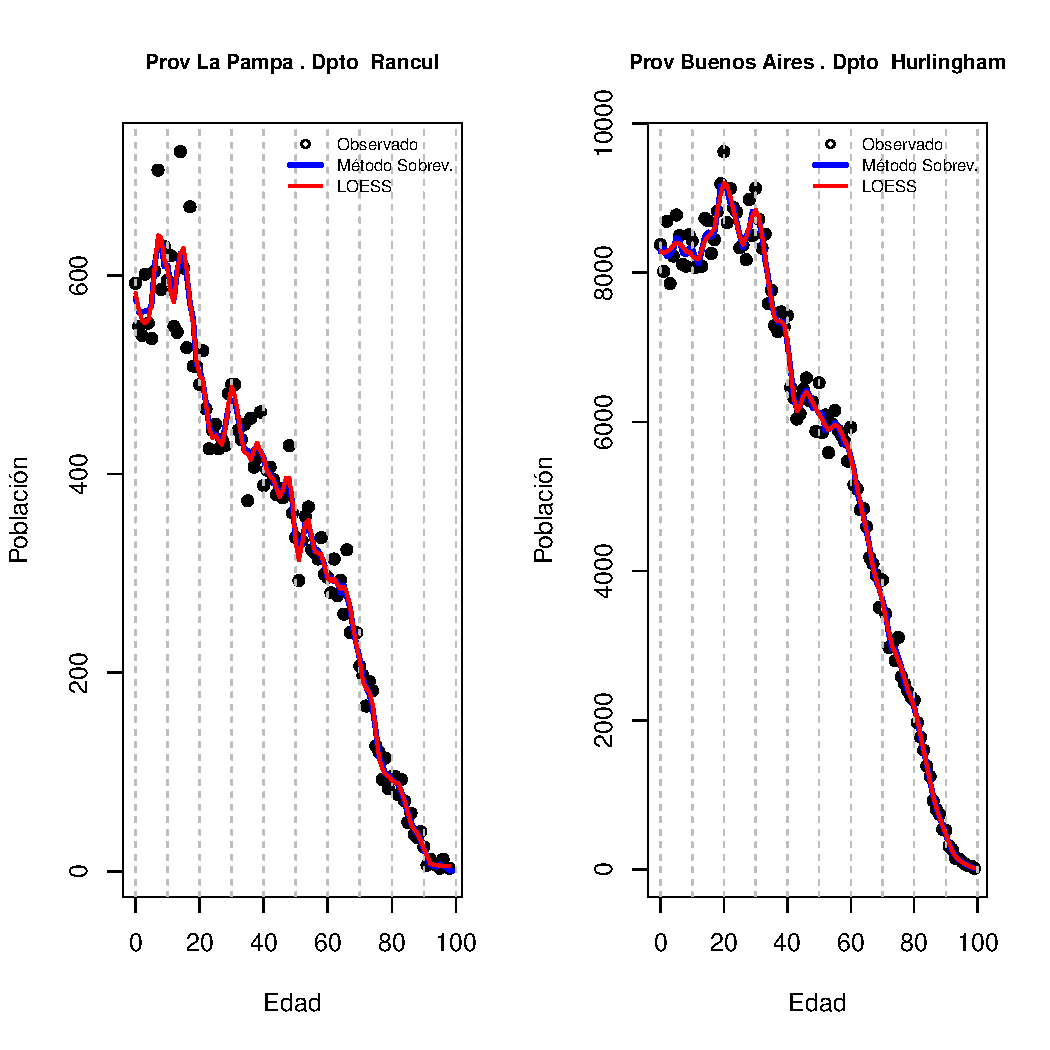
\includegraphics[width=0.7\linewidth]{/Users/nicosacco/GitHub/academicos/research/SubnMort/analysis/plots/AdjExp2} 

}

\caption{Ajuste de exposición 2008-2010. Dos casos. Fuente: elaboración propia en base a INDEC (2013)}\label{fig:AdjExp}
\end{figure}

\hypertarget{chequeos-de-consistencia}{%
\subsection{Chequeos de consistencia}\label{chequeos-de-consistencia}}

Se conocen diversas propuestas metodológicas para abordar el problema de
cobertura de muertes en áreas menores, dependiendo de la información
auxiliar con que se cuente (Preston et~al.
\protect\hyperlink{ref-Preston1980}{1980}; Bennett y Horiuchi
\protect\hyperlink{ref-Bennett_Horiuchi_1984}{1984}; Schmertmann y
Gonzaga \protect\hyperlink{ref-Schmertmann2018}{2018}; Alexander,
Zagheni, y Barbieri \protect\hyperlink{ref-Alexander2017}{2017}). La
utilización de métodos demográficos indirectos de evaluación de
cobertura son de difícil aplicación en una población pequeña muy
influenciada por la migración interna. Con el objetivo de visualizar
posibles problemas de datos en los departamentos, se realizaron dos
ejercicios.

Primero, se utilizó el método de Brass y Coale (Moultrie et~al.
\protect\hyperlink{ref-Moultrie}{2013}) para la estimación indirecta de
la mortalidad infantil y se mapeó con la esperanza de vida al nacer
(\(q_0\)) a partir de los datos de muerte, descritos en la sección
previa. Se trata de un método poco preciso para poblaciones pequeñas,
pero puede dar una idea sobre los problemas en las áreas mayores
(problemas relativos al numerador o denominador). En la Figura
\ref{fig:PF} observamos los puntos no ponderados y ponderados
poblacionalmente, con el fin de otorgar mayor relevancia a la
consistencia en las áreas más pobladas, responsables del posible sesgo
de suavizamiento en los procedimientos metodológicos, que serán
descritos en la siguiente sección. Utilizando la edad promedio de la
madre al nacimiento durante 2010 para cada provincia y la familia de
tablas de la Organización de Naciones Unidas (ONU) para América Latina,
de acuerdo a lo observado en la Figura \ref{fig:PF} concluimos que no
hay un sesgo claro en las áreas más mayores.

\begin{figure}

{\centering 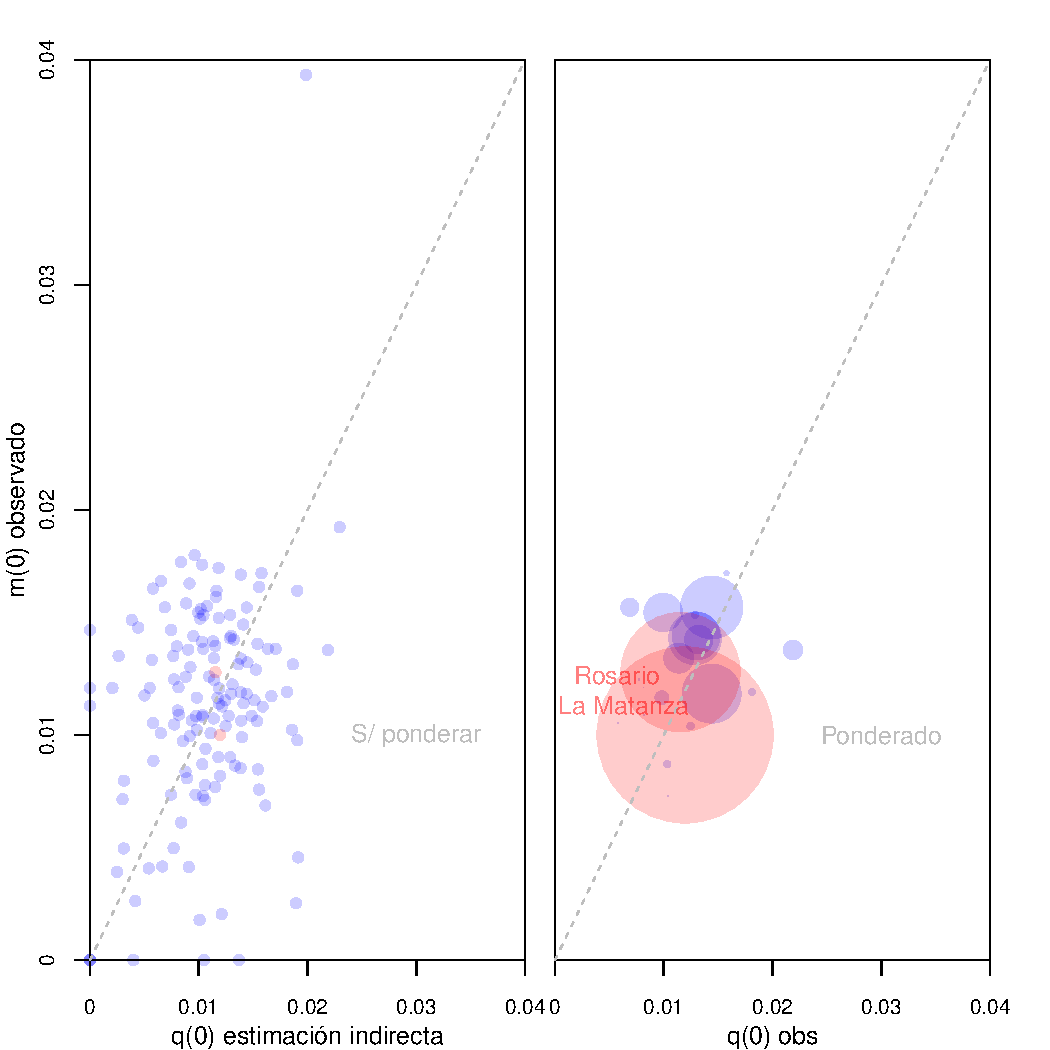
\includegraphics[width=0.7\linewidth]{/Users/nicosacco/GitHub/academicos/research/SubnMort/analysis/plots/ChekPF} 

}

\caption{Estimación indirecta de q(0) y tasa de mortalidad m(0) observada. Departamentos de la región Pampeana (excepto CABA). Fuente: elaboración propia en base a Censo y estadísticas vitales.}\label{fig:PF}
\end{figure}

En segundo lugar, se mapeó cada departamento respecto al indicador
censal de pobreza NBI (Necesidades Básicas Insatisfechas) elaborado por
el INDEC y la tasa de mortalidad general estandarizada a partir de la
estructura por edad regional, buscando una relación esperada (Kaztman
\protect\hyperlink{ref-Kaztman1995}{1995}; Preston
\protect\hyperlink{ref-Preston1975}{1975}; Grushka
\protect\hyperlink{ref-Grushka2013}{2013}). En el Cuadro \ref{fig:NBI}
se muestran el NBI4 y el NBI5, que miden el porcentaje de hogares con
niños en estado de inasistencia escolar y hogares con problemas de
subsistencia (hogares con cuatro o más personas por miembro ocupado y
que tienen un jefe que no ha completado el tercer grado de escolaridad
primaria) (Kaztman \protect\hyperlink{ref-Kaztman1995}{1995}). En color
se destaca el departamento más grande de la Región Pampeana, La Matanza
(que contiene al 10.7\% de la provincia de Buenos Aires). Este
departamento tiene una de las tasas de mortalidad estandarizadas más
bajas, pero un índice de pobreza similar (NBI4) o mayor (NBI5) al de los
demás. Si bien su desempeño en los índices de pobreza NBI1 (vivienda
inconveniente), NBI2 (carencias sanitarias) y NBI3 (hacinamiento) no es
reporta de manera tan marcada lo señalado, se decidió dejarlo fuera de
este artículo, debido principalmente a cuestiones metodológicas ya que
las áreas con mayor densidad poblacional son de extrema relevancia a la
hora de suavizar las menores y esto podría sesgar los resultados si es
que específicamente La Matanza tiene un problema.\footnote{INDEC
  advierte sobre los recuentos de población por departamento en el Censo
  2010, donde Buenos Aires fue una de las provincias con dificultades
  (\url{https://bit.ly/2R7svfX}, visitado el 10/1/2020)}

\begin{figure}

{\centering \includegraphics[width=0.7\linewidth]{/Users/nicosacco/GitHub/academicos/research/SubnMort/analysis/plots/ChekNBI} 

}

\caption{Tasa Estandarizada de mortalidad y NBI. Departamentos de Región Pampeana. Fuente: elaboración propia en base a censo y estadísticas Vitales}\label{fig:NBI}
\end{figure}

Se realizó un chequeo adicional de \(e_0\) para cada provincia (excepto
Buenso Aires\footnote{A partir de lo que resta del artículo, se
  considera a la provincia de Buenos Aires sin La Matanza.} debido la no
comparabilidad) a partir de los insumos anteriores y la estimación
oficial (INDEC \protect\hyperlink{ref-INDEC2013}{2013}). Los resultados
dan una diferencia relativa (\%) de 0,002, 0.39, 0.3, 0.98, 0.34 para
las provincias de Córdoba, Entre Ríos, La Pampa y Santa Fé. Por ende,
consideramos aceptable nuestra aproximación dado el año de distancia en
la referencia temporal y ya que no hemos realizado ajustes de cobertura
en la defunciones, aspecto que pudo haber sido realizado en las cifras
oficiales (Cuadro \ref{tab:Dif_e0_INDEC}, del Anexo).

\hypertarget{metodologuxeda}{%
\section{Metodología}\label{metodologuxeda}}

Debido a la relativa poca experiencia de estudios previos que estimen
mortalidad \emph{general} en áreas menores en Argentina, se decidió
aplicar tres técnicas: una basada en la teoría bayesiana, la segunda
basada en métodos relacionales de tablas de vida, pero adicionando
técnicas estadísticas de suavizamiento, y tercero una técnica indirecta.
Antes de la estimación, se realizó un procedimiento de regionalización
para aprovechar la similitud espacial entre áreas pequeñas,
independientemente de su pertenencia político-administrativa.

\hypertarget{regionalizaciuxf3n}{%
\subsection{Regionalización}\label{regionalizaciuxf3n}}

La definición de una región o cluster debe explorar la similitud interna
entre áreas pequeñas para poder suponer que su mortalidad es la
realización de un proceso estocástico mayor. La similitud en los
patrones de mortalidad suele abordarse por pertenecer a la misma
provincia, donde la ``distancia'' entre jurisdicciones no se mide por la
distancia geográfica o los atributos socioeconómicos (Longford
\protect\hyperlink{ref-Longford2005}{2005}).

Para ello, retomamos el enfoque propuesto por Assuncao et~al.
(\protect\hyperlink{ref-AssunCao2006}{2006}), que definió áreas mayores
internamente homogéneas y con condición de contigüidad en el espacio.
Primero se realizó un gráfico de conectividad entre los centroides y
luego se calculó el \emph{costo} entre ellos (distancia euclidiana en
nuestro caso). Luego, un procedimiento de iteración estimó el árbol de
expansión mínimo, que es el árbol conectado con un costo mínimo, medido
como la suma de las diferencias en todos los bordes. Finalmente, se
realizó un procedimiento de partición cortando el borde que minimiza la
varianza dentro de los dos grupos resultantes. Debido a que probar todas
las combinaciones posibles en cada partición es un problema
computacional, los autores propusieron un enfoque heurístico. Una
sobreclusterización aumentaría la homogeneidad pero también aumentaría
la varianza en las unidades más pequeñas debido a que no hay suficientes
casos. Esa es la razón para establecer umbrales mínimos de población o
áreas menores resultantes en cada parea mayor, siendo de veinte
departamentos el elegido en este caso.

Como insumos para el procedimiento de regionalización, utilizamos los
archivos \emph{shape} del INDEC disponibles en línea y el índice de NBI
del censo, ambos por departamento\footnote{\url{https://bit.ly/2sVpK9u},
  visitado el 10/01/2020.}. Se re-escaló el índice a unidades de
desviación estándar y aplicó la metodología comentada anteriormente,
implementada en el paquete \emph{spdep}, mediante la función
\emph{skater} (Bivand \protect\hyperlink{ref-Bivand2019}{2019}). El
resultado puede verse en Cuadro \ref{tab:table_e0} (del Anexo) y Cuadro
\ref{fig:cluster}.

Con esta segmentación en siete regiones se obtuvo un aumento de 14\% en
la varianza entre grupos y una disminución no tan importante de 1\% en
la varianza promedio dentro los grupos. La nueva fragmentación permitió
contar con grupos más dispares y con algo menos de variación relativa
interna.

\begin{figure}

{\centering \includegraphics[width=0.7\linewidth]{/Users/nicosacco/GitHub/academicos/research/SubnMort/analysis/plots/cluster} 

}

\caption{Regionalización de departamentos. Fuente: elaboración propia en base a Censo y Estadísticas Vitales}\label{fig:cluster}
\end{figure}

\hypertarget{muxe9todos-de-estimaciuxf3n}{%
\subsection{Métodos de estimación}\label{muxe9todos-de-estimaciuxf3n}}

Aunque Argentina generalmente se clasifica como un país con buenas
estadísticas estadísticas vitales (Jaspers y Orellana
\protect\hyperlink{ref-JaspersOrellana1994}{1994}; Luy
\protect\hyperlink{ref-Luy2010}{2010}), se conoce que hay un porcentaje
desigual de muertes infantiles no registradas por provincia (DEIS
\protect\hyperlink{ref-DEIS2016}{2016}). En este sentido, dado que la
fuente de datos es un registro, y pensando en la estimación de las tasas
de mortalidad por edad, se podría concluir que no habría varianza, y que
el sesgo (ambos componentes del error cuadrado medio de un estimador)
vendría dado por el patrón de casos omitidos en cada jurisdicción. Como
se mencionó anteriormente, este segundo componente del error no se
abordará en este trabajo debido a que no hay información sobre su
distribución por áreas pequeñas. Con respecto al primero, pese a lo
mencioando, existen fenómenos con un pequeño número de ``experimentos''
(pocos expuestos en nuestro caso), que tienen una mayor variación en sus
estimaciones, por lo que requiere un tratamiento especial para reflejar
el riesgo de mortalidad subyacente (Brillinger
\protect\hyperlink{ref-Brillinger1986}{1986}). Para lograrlo, utilizamos
tres métodos diferentes, los cuales se diferencian en la forma en que
las áreas menores \emph{toman prestada} información del área mayor que
las contiene.

El método empírico bayesiano mejora la eficiencia estadística de los
estimadores de las tasas de mortalidad por edad, disminuyendo la
varianza en los casos de jurisdicciones pequeñas (Efron y Morris
(\protect\hyperlink{ref-Efron1972}{1972}); Marshall
(\protect\hyperlink{ref-Marshall1991}{1991}); Longford
(\protect\hyperlink{ref-Longford2005}{2005}); Assunção et~al.
(\protect\hyperlink{ref-Assuncao2005}{2005})). La idea es que,
suponiendo que las diferentes observaciones de cada área procedan de una
distribución \emph{a priori} común, cada estimación se puede mejorar
utilizando la información de las otras. La distribución \emph{a priori}
corresponde a la distribución conjunta del vector de tasas de mortalidad
por edad del área mayor. Luego, a través del comportamiento observado en
cada área menor, se produce el ajuste bayesiano de la distribución de
mortalidad \emph{a posteriori}. La característica de ``empírico'' radica
en que las distribuciones de los parámetros del área mayor se estiman
también a partir de los datos observados, en este caso por el método de
los momentos.

Veamos primero el caso univariable. Considerando un grupo de edad de
cinco años, ya sea en un área \(i\), se supone que la distribución de
muertes \(d\) es un proceso de Poisson, con una media esperada de
\(E(d_ {x,4}^{i}|{m_{x,4}^{i}})=N_{x,4}^{i}m_{x,4}^{i}\), siendo \(N\)
las exposiciones y \(m\) la tasa de mortalidad.

Primero se considera a \(\hat{m}_{x,4}^{i}=D_{x,4}^{i}/N_{x,4}^{i}\)
como el estimador de máxima probabilidad de la tasa \(m_{x,4}^{i}\) en
el área \(i\), que son \(iid\) generados a partir de \(m_{x,4}\). La
esperanza condicionada de \(\hat{m}_{x,4}^{i}\) es
\(E_{m}(E({\hat{m}}_{x,4}^{i})/m_{x,4}^{i})=E_{m}({m_{x, 4}^{i}}) = m_{x,4}\)
(tasa de área grande) y la varianza condicionada
\(V({\hat{m}}_{x,4}^{i}/m_{x,4}^{i})=\frac{m_{x,4}^{i}}{N_{x,4}^{i}}\).

La varianza total del estimador se puede expresar como la suma de la
varianza de las medias de \$ i's \$ y la esperanza de las varianzas de
\(i's\):
\(V_{m}(E(\hat{m}_{x,4}^{i}/m_{x,4}^{i}))+E_{m}(V({\hat{m}}_{x,4}^ {i}/m_{x,4}^{i}))=V_{m}(\hat{m}_{x,4}^{i})+E_{m}(\frac{{\hat{m}}}{N_{x,4}^{i}})=V_{m}(m_{x,4}^{i})+\frac{m_{x, 4}}{N_{x,4}^{i}}\).
Eso está relacionado con la relación jerárquica entre el hiperparámetro
(\(m_{x, 4}\)), los parámetros (\(m_{x,4}^{i}\)) y sus estimadores
\(\hat{m}_{x,4}^{i}\).

El estimador lineal bayesiano \(\mathring{m}_{x, 4}^{i}\) que minimiza
el error cuadrático medio de \({m}_{x,4}^{i}\) (e indicadores que son
funciones lineales de esto) está dado por la siguiente fórmula, de
acuerdo a (\protect\hyperlink{ref-Robbins1983}{1983}):

\[\mathring{m}_{x,4}^{i}=\hat{m}_{x, 4}^{i}+S_{x,4}^{i}(\bar{m}_{x,4}^{i}-\hat{m}_{x,4}^{i})\]

Nuevamente, es empírico porque \(m_{x,4}\) se estima por método de
momentos con \(\bar{m}_{x,4}\), la media ponderada de áreas pequeñas. El
factor de ``contracción'' \(S_{x, 4}^{i}\) (``shrinkage'' en la
bibliografía) es la relación entre la expectativa de la varianza
estimada en el área pequeña \(i\) y la varianza no condicionada del
estimador, que es:

\[S_{x,4}^{i}=\frac{V_{m}(m_{x,4}^{i})}{V_{m}(m_{x,4}^{i})+\frac{m_{x,4}}{N_{x,4}^{i}}}\]

Visto de otra manera, esta fórmula representa la relación entre la
varianza del área más pequeña con respecto a la suma de la varianza
total (del área más pequeña y más grande), en sintonía con un análisis
de la varianza clásica entre grupos (ANOVA). Siguiendo este
razonamiento, en un contexto de extrema homogeneidad, un área menor muy
pequeña podría caracterizarse a partir de la estimación del área más
grande (\(S_{x, 4} ^ {i} \cong 1\)). Por otro lado, las áreas de alto
peso poblacional tomarán valores cercanos a los observados
(\(S_{x,4}^{i}\cong 0\)). En el medio de estos extremos, la función
combina linealmente la estimación del área grande con respecto al área
más pequeña incluida.

Longford (\protect\hyperlink{ref-Longford1999}{1999}) extendió esta idea
a vectores de variables aleatorias (``contracción multivariada''),
estimando \(S_{x,4}^{i}\) de manera de aprovechar la correlación entre
subpoblaciones. En nuestro caso, si la tasa de mortalidad del grupo de
edad entre \(x\) y \(x+4\) del área \(i\) es mayor que el área \(j\),
una correlación alta implicaría que en edades contiguas ocurriría lo
mismo con mayor probabilidad. Si la covarianza fuera nula, este enfoque
sería equivalente al caso univariante descrito anteriormente. Los
cálculos realizados en este trabajo se realizaron para edades de 0, 1-4
y quinquenales hasta el grupo de edad abierta 80. El desarrollo se
realizó siguiendo el enfoque mostrado en Assunção et~al.
(\protect\hyperlink{ref-Assuncao2005}{2005}), que estimó los parámetros
por el método de momentos para las tasas de fecundidad en Brasil.

El otro método aplicado se basó en un modelo de mortalidad relacional
llamado TOPALS (Tool for Projecting Age-Specific rates using Linear
Splines) (Beer (\protect\hyperlink{ref-deBeer2011}{2011})), que utiliza
un método spline lineal para describir los ratios entre las
probabilidades de muerte por edad de una población dada y un patrón. Una
ventaja contra el enfoque logit clásico de Brass es que TOPALS es menos
sensible al elegir el estándar. Gonzaga y Schmertmann
(\protect\hyperlink{ref-Gonzaga_Schmertmann_2016}{2016}) incluyeron esta
idea en una regresión de Poisson en las tasas de mortalidad por edad
simple, permitiendo intervalos de confianza para los resultados que
tienen en cuenta la varianza por razones de baja exposición.

Específicamente, el vector de tasas de mortalidad en el área pequeña
\(m^{i}(\alpha) = m^{*}*\exp^{\alpha B_{x}}\) es una función de los
``nodos'' spline \(\alpha\), que son las edades en las que se evaluará
el desvío respecto al patrón estándar, siendo \(m^*\) el vector de tasa
de mortalidad estándar, y \(B_{x}\) es la matriz B-spline que
multiplicada por \(\alpha\) brinda el desplazamiento lineal entre el
logaritmo de ambas tasas.

La idea es suponer que \(D_{x}\sim Poi (m_ {x} N_ {x})\) en cada área
pequeña, construir la función de probabilidad usando las muertes y
exposiciones observadas
\(\log(L(m_{x}N_{x}|D_{x}))=\sum_{\forall x}{\lbrack -m_{x}N_{x}+D_{x}\ln (m_{x})+D_{x}\ln (N_{x})-\ln (D_{x}!)\rbrack}\),
pero expresando eso en función del parámetro \(\alpha\), agregando una
penalización por distancia desde el estándar y suavizando entre edades
adyacentes. Se colocan nodos en edades más determinantes en el perfil de
mrotalidad, para luego minimizar el log-likelihood:
\(Q(\alpha )=\sum_{\forall x}{\lbrack -m(\alpha )_{x}N_{x}+D_{x}\ln(m(\alpha )_{x})\rbrack }-\sum_{k=0}^{5}{(\alpha _{k}-\alpha _{k+1})^{2}}\).

El método empírico bayesiano es particularmente apropiado en casos con
pequeñas pocos casos locales, variaciones regionales significativas,
altas correlaciones entre los componentes y relaciones espaciales
conocidas (Assunção et~al. \protect\hyperlink{ref-Assuncao2005}{2005}).
En el caso de la regresión TOPALS, la aplicación es más una técnica de
suavización que un modelo de variabilidad espacial, por lo que se
necesitan menos supuestos sobre las relaciones entre áreas.

Finalmente, como método básico, se aplicará el método de estandarización
indirecta, quizás uno de los primeros enfoques para este problema
(Arriaga \protect\hyperlink{ref-Arriaga2011}{2011}). Se basa en cambiar
solo el nivel del área principal para replicar las muertes observadas
del área menor que se está estimando. Podría catalogarse como el más
restrictivo de los modelos relacionales, aquel en el que no se tiene en
cuenta ninguna información sobre la forma de la mortalidad por edad del
área menor.

\hypertarget{resultados}{%
\section{Resultados}\label{resultados}}

Las estimaciones se calcularon para grupos quinquenales de edad (excepto
el primer grupo, separado en 0 y 1-4) con 90 y más como grupo abierto
final, en todos los departamentos de la Región Pampeana (excepto La
Matanza y aquellos en CABA, por motivos ya expuestos). El método TOPALS
fue pensado para ser aplicado en edades simples, pero en este caso
debido a que no se corrigió la omisión en áreas pequeñas y con motivo de
ser comparable con los demás métodos, se aplicó a edades quinquenales
tomando nodos en los grupos 0, 5-9, 20-24, 40-44 y 60-64. En el Cuadro
\ref{fig:Ajuste} se muestran cuatro ejemplos de ajuste.

\begin{figure}

{\centering 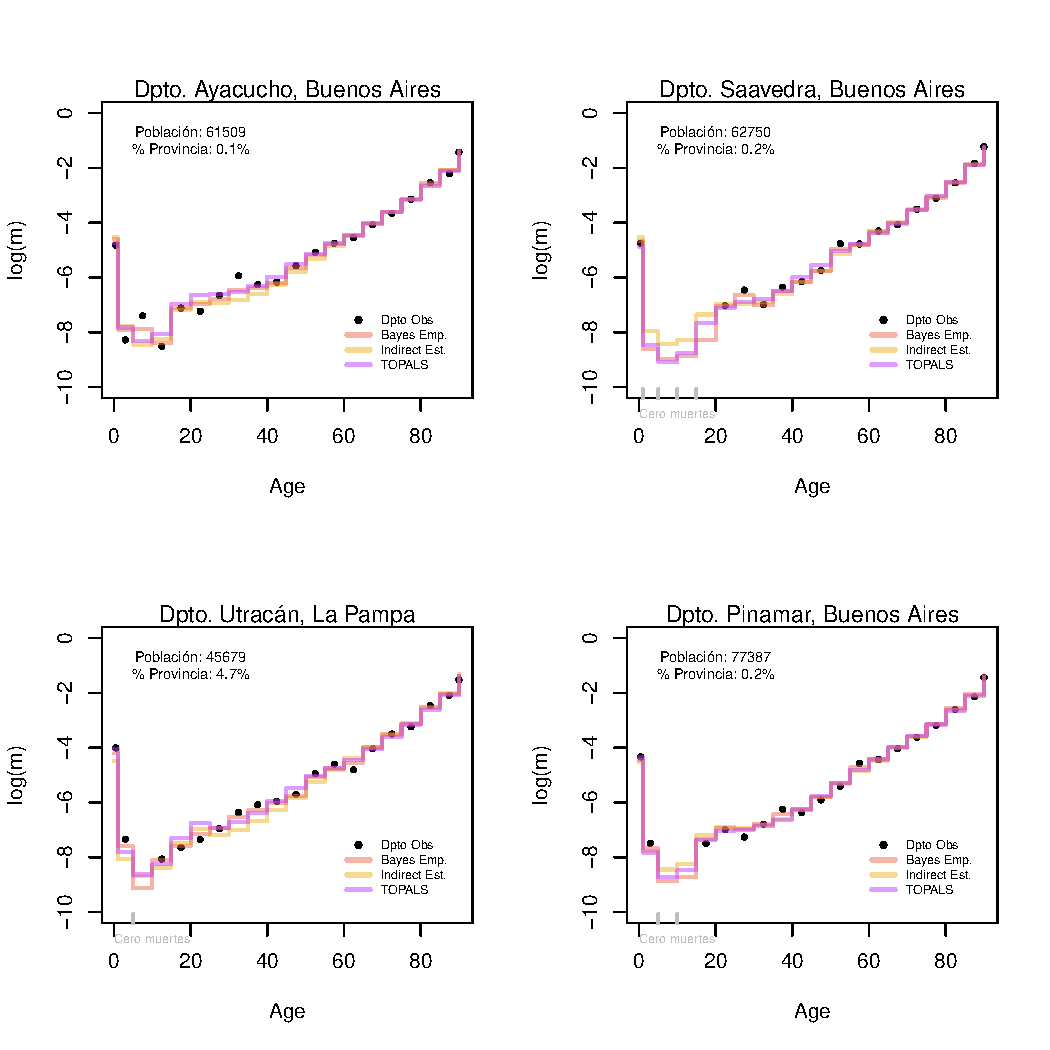
\includegraphics[width=0.7\linewidth]{/Users/nicosacco/GitHub/academicos/research/SubnMort/analysis/plots/Ajuste2} 

}

\caption{Estimación de la mortalidad por grupos de edad en departamentos de la Regiónn Pamepana, según método. Cuatro Casos. Fuente: elaboración propia en base a censo y estadísticas vitales.}\label{fig:Ajuste}
\end{figure}

Tomaremos \(e_0\) debido a que es la medida resumen más aceptada para
comparar el nivel de mortalidad entre poblaciones a un momento
determinado, y con fines conservadores debido a que el efecto de
posibles problemas en edades adultas mayores (con mayor variabilidad en
áreas pequeñas debido a su tamaño) tienen poco efecto en las
estimaciones sobre \(e_0\) en poblaciones donde la mortalidad infantil y
juvenil puedan tener un peso relevante en el indicador (Wrycza y
Baudisch \protect\hyperlink{ref-Wrycza2012}{2012}).

Por un lado, la correlación entre los métodos es clara: existe una gran
similitud entre TOPALS y la estimación indirecta (0.97), pero menor en
Bayes Empírico contra la estimación indirecta (0.84) y TOPALS (0.88)
(Cuadro \ref{fig:comparativeMeth}). Las principales diferencias se deben
a que el método bayesiano tiende a tomar \emph{siempre} alguna
información sobre el patrón de edad, suponiendo una correlación entre
edades contiguas dado el comportamiento global del área mayor. En los
dos restantes métodos, el patrón stándard es de mayor fuerza
gravitatoria. Los departamentos donde se reportan las mayores
diferencias son aquellos con pocas celdas distintas de cero (ver Cuadro
\ref{fig:Feos} en el Anexo).

\begin{figure}

{\centering 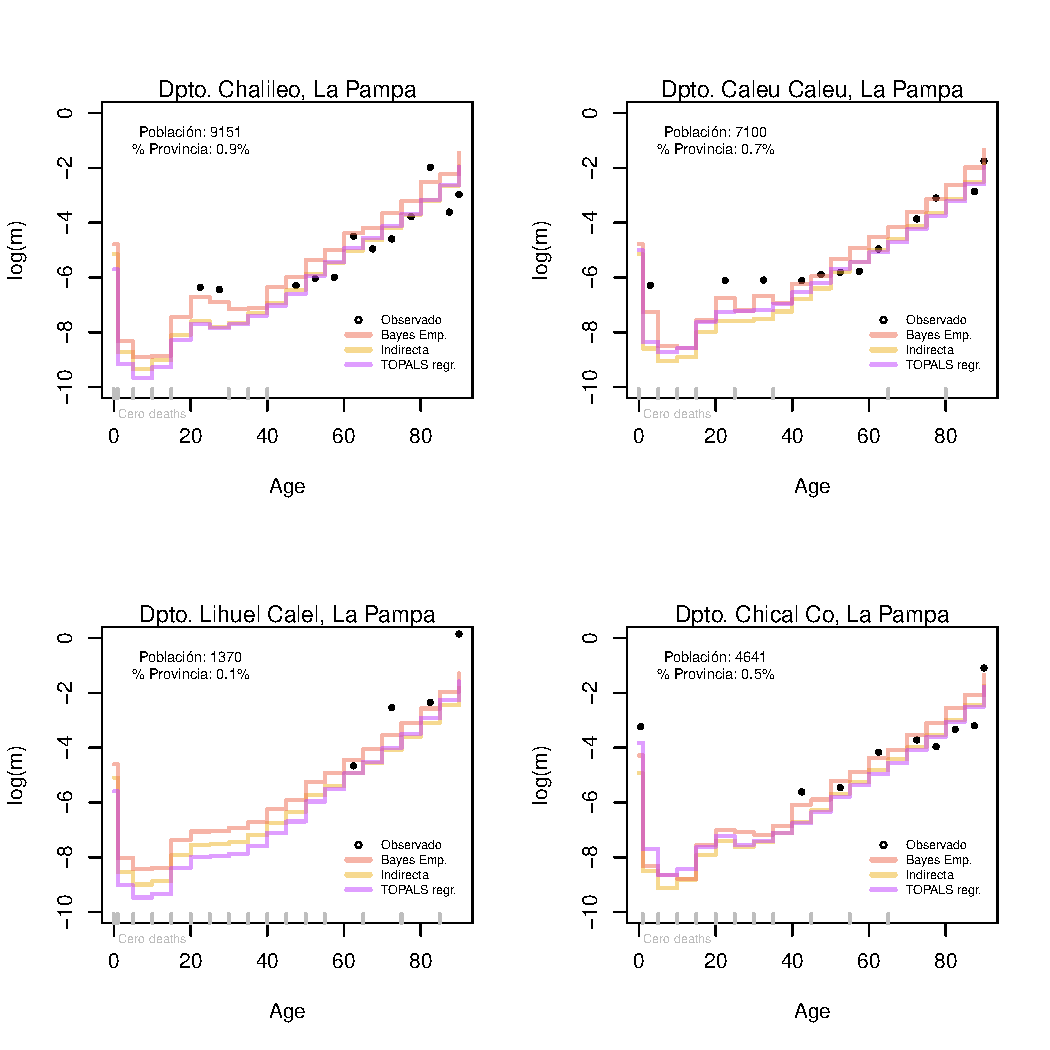
\includegraphics[width=0.7\linewidth]{/Users/nicosacco/GitHub/academicos/research/SubnMort/analysis/plots/AjusteFeos2} 

}

\caption{Estimaciones de mortalidad de los departamentos con mayores diferencias entre métodos. Fuente: elaboración porpia}\label{fig:Feos}
\end{figure}

Por otro lado, se siguió el procedimiento empleado por Gonzaga y
Schmertmann (\protect\hyperlink{ref-Gonzaga_Schmertmann_2016}{2016}),
relacionando las defunciones del área mayor con las obtenidas mediante
la agregación de las estimaciones para las áreas menores, en nuestro
caso las siete regiones (Cuadro \ref{fig:consistAM}, del Anexo). Si bien
los promedios de diferencias relativas son 0.3\%, 0.3\%, -0.1\% para los
métodos Indirecto, Bayesiano y TOPALS, se destaca mayor variabilidad en
el segundo y tercero (especialmente en las regiones 5 y 6, siempre menor
al 6\% en primeras edades), y un patrón singular en el primero que
sugiere un sesgo específico en algunos grupos (diferencia positivas y
negativas cruzando el eje x en edades alrededor de 60, en regiones 1, 3
y 7).

En el Cuadro \ref{fig:jerarq} se consideraron los resultados del método
de bayesiano debido a presentar un escenario más conservador en el rango
de estimaciones (futuras líneas de investigación deberían utilizar
técnicas de simulación para llegar a conclusiones más sólidas, como se
menciona al final del trabajo). Para tener en cuenta la aleatoriedad, se
realizó un proceso bootstrap de los recuentos de muertes a partir de una
distribución de Poisson en cada grupo etario. Esto permitió contar con
percentiles de las funciones de la tabla de vida y específicamente de la
esperanza de vida al nacer (ver Cuadro \ref{fig:jerarq} y tabla
\ref{tab:table_e0}, donde se muestran las estimaciones en el intervalo
de 95\%).

\begin{figure}

{\centering \includegraphics[width=0.48\linewidth]{/Users/nicosacco/GitHub/academicos/research/SubnMort/analysis/plots/BA} \includegraphics[width=0.48\linewidth]{/Users/nicosacco/GitHub/academicos/research/SubnMort/analysis/plots/Córdoba} \includegraphics[width=0.48\linewidth]{/Users/nicosacco/GitHub/academicos/research/SubnMort/analysis/plots/ER} \includegraphics[width=0.48\linewidth]{/Users/nicosacco/GitHub/academicos/research/SubnMort/analysis/plots/Santa_Fe} \includegraphics[width=0.48\linewidth]{/Users/nicosacco/GitHub/academicos/research/SubnMort/analysis/plots/La_Pampa} 

}

\caption{Estimaciones de mortalidad por Provincia según departamentos. Fuente: elaboración porpia}\label{fig:jerarq}
\end{figure}

Puede verse que el ancho del intervalo se encuentra relacionado con el
peso poblacional. Considerando esto, en el caso de Córdoba podemos decir
que mientras Calamuchita poseía un promedio de años de vida al nacer de
entre 77 y 78.3, Sobremonte poseía un promedio entre 73 y 75, con dos
años de diferencia considerando los límites inferiores y superiores
respectivamente. Futuros trabajos que relacionen ecológicamente estas
medidas pueden potenciar el análisis socio-económico de las jerarquías
halladas.

\begin{table}

\caption{\label{tab:dispersion}Resumen de estimaciones por provincia. Esperanza de vida al nacer. Región Pampeana. Años 2009-2011}
\centering
\begin{tabular}[t]{lrrrr}
\toprule
Provincia & Promedio & n & Varianza & Rango\\
\midrule
Buenos Aires & 75.7 & 134 & 1.4 & 6.3\\
Córdoba & 76.1 & 27 & 0.6 & 3.5\\
Entre Ríos & 75.1 & 18 & 0.5 & 2.2\\
La Pampa & 76.9 & 23 & 0.4 & 2.7\\
Santa Fé & 75.4 & 20 & 1.1 & 3.4\\
\bottomrule
\multicolumn{5}{l}{\textsuperscript{a} El promedio y varianza no estan ponderados por}\\
\multicolumn{5}{l}{población.}\\
\multicolumn{5}{l}{\textsuperscript{b} Buenos Aires no incluye La Matanza.}\\
\multicolumn{5}{l}{\textsuperscript{c} Fuente: elaboración propia en base a censo y}\\
\multicolumn{5}{l}{estadísticas vitales.}\\
\end{tabular}
\end{table}

Los resultados a su vez indican que la provincia de Buenos Aires fue la
de mayor dispersión medida por el rango (distancia entre máximo y
mínimo) y la varianza de los promedios (no ponderada poblacionalmente),
como por el coeficiente de variación. Luego se ubica Santa Fé con un un
ragno de 3.4, similar a Córdoba, pero con una varianza mayor para un un
promedio menor.

\hypertarget{la-provincia-de-buenos-aires}{%
\subsection{La provincia de Buenos
Aires}\label{la-provincia-de-buenos-aires}}

¿Qué nos permiten decir las estimaciones? Buenos Aires es la provincia
más poblada de Argentina, conteniendo 135 áreas administrativas. En la
tabla previa \ref{tab:dispersion} se mostró su gran heterogeneidad
(considerando 134 departamentos), con un rango estimado de esperanza de
vida al nacer de más de 6 años. La provincia se puede dividir entre el
área del Gran Buenos Aires compuesta por 24 departamentos (área urbana
que rodea a CABA) y el resto de la superficie, con características muy
disímiles. Para inspeccionar un poco el significado de los resultados,
en el Cuadro \ref{fig:dptosBsAs} describimos tres jurisdicciones con
exposición significativa y ubicadas a lo largo de la distribución: San
Isidro, General Pueyrredón y Moreno.

\begin{figure}

{\centering \includegraphics[width=0.48\linewidth]{/Users/nicosacco/GitHub/academicos/research/SubnMort/analysis/plots/SanIsyMoreno} 

}

\caption{Tasas de mortalidad según áreas seleccionadas de la Provincia de Buenos Aires. Fuente: elaboración propia}\label{fig:dptosBsAs}
\end{figure}

Si comparamos la mediana de las tasas por edad, Moreno presenta una
mayor mortalidad infantil pero también un mayor riesgo en adultos
mayores. \emph{A priori}, no hay ninguna razón para creer en una
exposición con omisión diferencial en mayores de 40 años de edad, por lo
que probablemente este sea un patrón de mortalidad a tener en cuenta. En
el caso de San Isidro, con la mayor esperanza de vida al nacer de este
grupo, presentó la curva más baja en el rango de edad típico de causas
externas. Finalmente, Gral. Pueyrredón tuvo la peor posición en el rango
de edad de 5 a 25 años, edades con un porcentaje importante de
mortalidad por causas prevenibles. En términos estadísticos, dado el
modelo empleado, los rangos de edad donde se pueden ensayar
comparaciones jerárquicas entre las tres jurisdicciones tomadas son
aquellos donde los polígonos no se solapan: infantil y adulta mayor a 45
años, y 15-24 entre San Isidro y Gral. Pueyrredón.

\hypertarget{limitaciones-y-trabajo-futuro}{%
\section{Limitaciones y Trabajo
futuro}\label{limitaciones-y-trabajo-futuro}}

Una de las limitaciones de esta propuesta es que se desconoce el nivel
de cobertura de las áreas menores. Se realizó un análisis de datos
desconocidos en el registro de defunciones y algunas comprobaciones
visuales sobre la consistencia entre un indicador censal socioeconómico
(NBI) y estimaciones indirectas de mortalidad infantil con el fin de
detectar posibles anomalías, pero solo enfocándose en los departamentos
de gran volumen debido a las propiedades estadísticas de los métodos. El
costo fue grande: se dejó fuera de la estimación al departamento más
grande del país y a la Ciudad Autónoma de Buenos Aires, y no se
desagregó por sexo el ejercicio. Correcciones sobre los datos deben
realizarse a partir de información externa si se deciden incorporar en
futuras investigaciones que apliquen al período considerado.

En investigaciones ulteriores, otros análisis serán necesarios. Por un
lado, para realizar una comparación metodológica robusta podrían
simularse perfiles de mortalidad según tablas modelo, en diferentes
escalas y patrones de omisión, incorporando otros desarrollos recientes
al análisis (por ejemplo Alexander
(\protect\hyperlink{ref-Alexander2017}{2017})). Por otro lado, el censo
de población próximo (ronda 2020) permitirá realizar este ejercicio
dando pautas para apoyar o no la hipótesis de convergencia señalada en
la introducción.

\hypertarget{conclusiones}{%
\section{Conclusiones}\label{conclusiones}}

Los antecedentes de estimación en áreas pequeñas son escasos en
Argentina. Decidimos comenzar con la Región Pampeana debido a su
participación poblacional del país. Aplicamos tres métodos para estimar
la estructura y el nivel de mortalidad, y realizamos verificaciones de
consistencia previas para descartar grandes problemas. Las principales
diferencias entre los métodos se deben a que el método bayesiano
empírico tiende a tomar siempre alguna información sobre el patrón de
edad del área menor, pero a su vez con un poco de menor consistencia en
lo agregado. Se ensayó un análisis comparativo para el caso de Buenos
Aires, caracterizando tres departamentos y cuantificando diferentes
perfiles de mortalidad, aunque con reparos estadísticos.

En la búsqueda de información sobre heterogeneidad intraprovincial en la
mortalidad hay decisiones que tomar en el numerador y denominador de las
tasas por edad. Hay un límite en lo que podemos concluir, pero resulta
necesario remarcar cuestiones relativas a aquellas áreas en desventaja.
Este puede ser un punto de partida para dar prioridades en el diseño de
políticas de salud a nivel local y dar pie a futuras investigaciones que
aporten tanto sobre la calidad de datos como en los aspectos
metodológicos de áreas menores.

\hypertarget{anexo}{%
\subsection{Anexo}\label{anexo}}

\begin{landscape}\begin{table}

\caption{\label{tab:SinDEP}Provincias según Departamento de residencia desconocido. Región Pampeana. Años 2009-2011}
\centering
\begin{tabular}[t]{lr}
\toprule
Provincia & Desconocido \%\\
\midrule
Ciudad Autónoma de Buenos Aires & 8.6\\
Buenos Aires & 0.9\\
Catamarca & 0.7\\
Córdoba & 0.3\\
Corrientes & 1.0\\
\addlinespace
Chaco & 0.8\\
Chubut & 1.5\\
Entre Ríos & 0.7\\
Formosa & 0.9\\
Jujuy & 3.1\\
\addlinespace
La Pampa & 1.6\\
La Rioja & 0.7\\
Mendoza & 0.4\\
Misiones & 0.8\\
Neuquén & 0.7\\
\addlinespace
Río Negro & 1.7\\
Salta & 0.6\\
San Juan & 0.7\\
San Luis & 1.4\\
Santa Cruz & 2.4\\
\addlinespace
Santa Fe & 0.4\\
Santiago del Estero & 1.2\\
Tucumán & 1.7\\
Tierra del Fuego, Antártida e Islas del Atlántico Sur & 2.5\\
\bottomrule
\multicolumn{2}{l}{\textsuperscript{a} Fuente: elaboración propia}\\
\end{tabular}
\end{table}
\end{landscape}

\begin{landscape}\begin{table}

\caption{\label{tab:UnkSexAge}Departamentos con mayor porcentaje de información desconocida en sexo y edad. Región Pampeana. Años 2009-2011}
\centering
\begin{tabular}[t]{llrllr}
\toprule
Provincia & Departamento & \% Edad & Provincia & Departamento & \% Sexo\\
\midrule
Buenos Aires & General Alvear & 2.2 & Buenos Aires & General Pueyrredón & 7.3\\
Buenos Aires & Leandro N. Alem & 1.9 & Buenos Aires & Vicente López & 5.6\\
Buenos Aires & General La Madrid & 1.8 & Buenos Aires & Quilmes & 3.8\\
Buenos Aires & General Pinto & 1.6 & Buenos Aires & Coronel Dorrego & 3.7\\
Buenos Aires & Las Flores & 1.6 & Buenos Aires & Ituzaingó & 3.1\\
\addlinespace
Buenos Aires & Maipú & 1.6 & Buenos Aires & San Andrés de Giles & 2.5\\
Buenos Aires & Florentino Ameghino & 1.4 & Buenos Aires & Bahía Blanca & 2.4\\
Buenos Aires & Salliqueló & 1.4 & Buenos Aires & General San Martín & 2.3\\
Buenos Aires & Castelli & 1.2 & Buenos Aires & San Miguel & 2.2\\
Buenos Aires & Pellegrini & 1.2 & Buenos Aires & La Plata & 2.1\\
\bottomrule
\multicolumn{6}{l}{\textsuperscript{a} Fuente: elaboración propia}\\
\end{tabular}
\end{table}
\end{landscape}

\begin{landscape}\begin{table}

\caption{\label{tab:def_tardias}Distribución de defunciones registradas y ocurridas. Región Pampeana. Años 2009-2011}
\centering
\begin{tabular}[t]{lrrrrrr}
\toprule
\multicolumn{1}{c}{ } & \multicolumn{6}{c}{Año de ocurrencia} \\
\cmidrule(l{3pt}r{3pt}){2-7}
  & 2008 & 2009 & 2010 & 2011 & 2012 & 2013\\
\midrule
2009 & 0.94 & 99.06 & 0.00 & 0.00 & 0.00 & 0.00\\
2010 & 0.00 & 0.79 & 99.21 & 0.00 & 0.00 & 0.00\\
2011 & 0.00 & 0.00 & 1.12 & 98.88 & 0.00 & 0.00\\
2012 & 0.00 & 0.00 & 0.00 & 1.13 & 98.87 & 0.00\\
2013 & 0.00 & 0.00 & 0.00 & 0.00 & 1.29 & 98.71\\
\bottomrule
\multicolumn{7}{l}{\textsuperscript{a} El año de registro está en las filas y el de ocurrencia en}\\
\multicolumn{7}{l}{las columnas. Fuente: elaboración propia}\\
\end{tabular}
\end{table}
\end{landscape}

\begin{landscape}\begin{table}

\caption{\label{tab:Dif_e0_INDEC}Diferencias entre la esperanza de vida calculada con datos no ajustados y estimaciones oficiales. Región Pampeana. Años 2009-2011}
\centering
\begin{tabular}[t]{llrrr}
\toprule
  & Provincia & Propia & INDEC & Dif.(\%)\\
\midrule
2 & Cordoba & 76.05 & 75.75 & 0.39\\
3 & Entre Rios & 75.20 & 74.98 & 0.30\\
4 & La Pampa & 76.95 & 76.20 & 0.98\\
5 & Santa Fe & 75.36 & 75.10 & 0.34\\
\bottomrule
\multicolumn{5}{l}{\textsuperscript{a} Fuente: elaboración propia}\\
\end{tabular}
\end{table}
\end{landscape}

\begin{figure}

{\centering 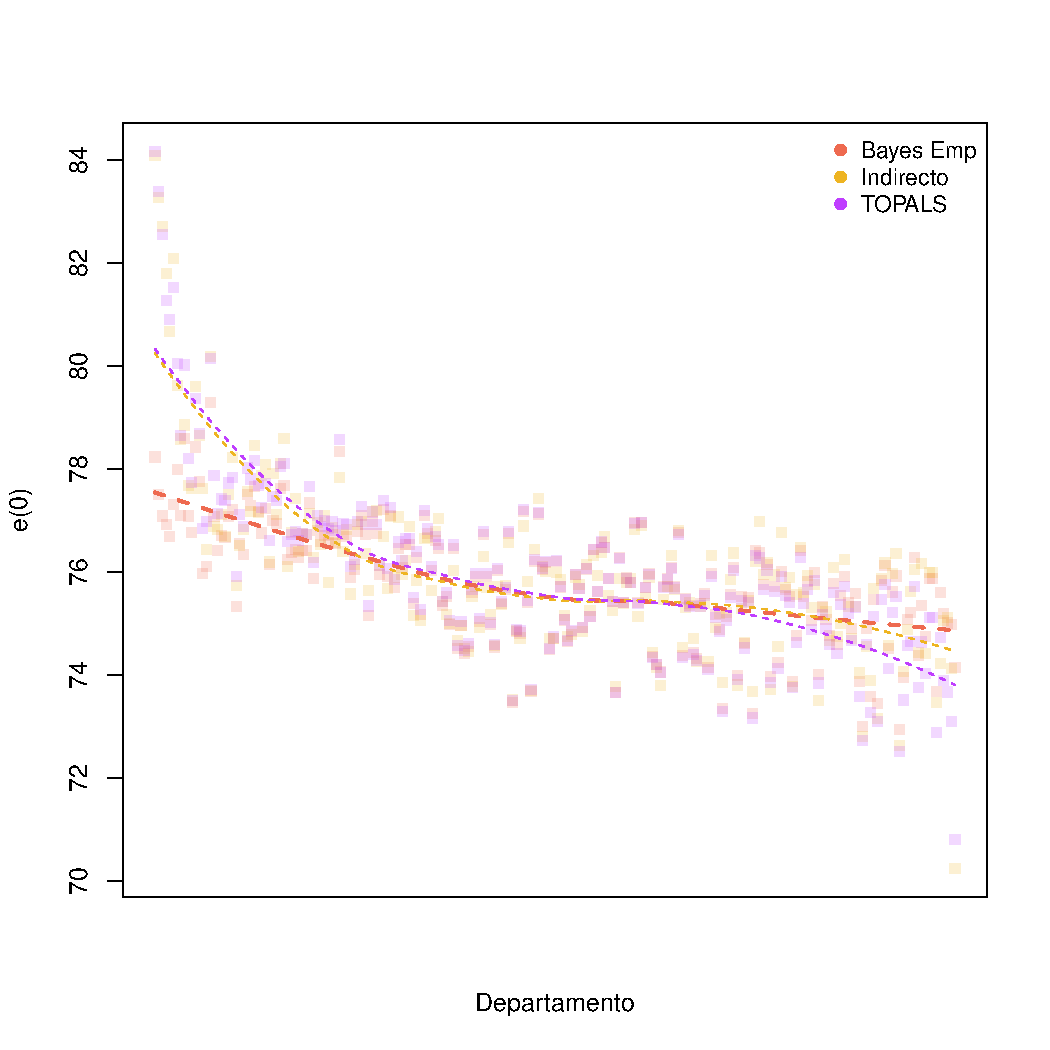
\includegraphics[width=0.7\linewidth]{/Users/nicosacco/GitHub/academicos/research/SubnMort/analysis/plots/CompMethods} 

}

\caption{Estimaciones de esperanza de vida al nacer según tres metodologías. Cada punto corresponde a un departamento. Fuente: elaboración propia en base a censo y estadísticas vitales.}\label{fig:comparativeMeth}
\end{figure}

\begin{figure}

{\centering 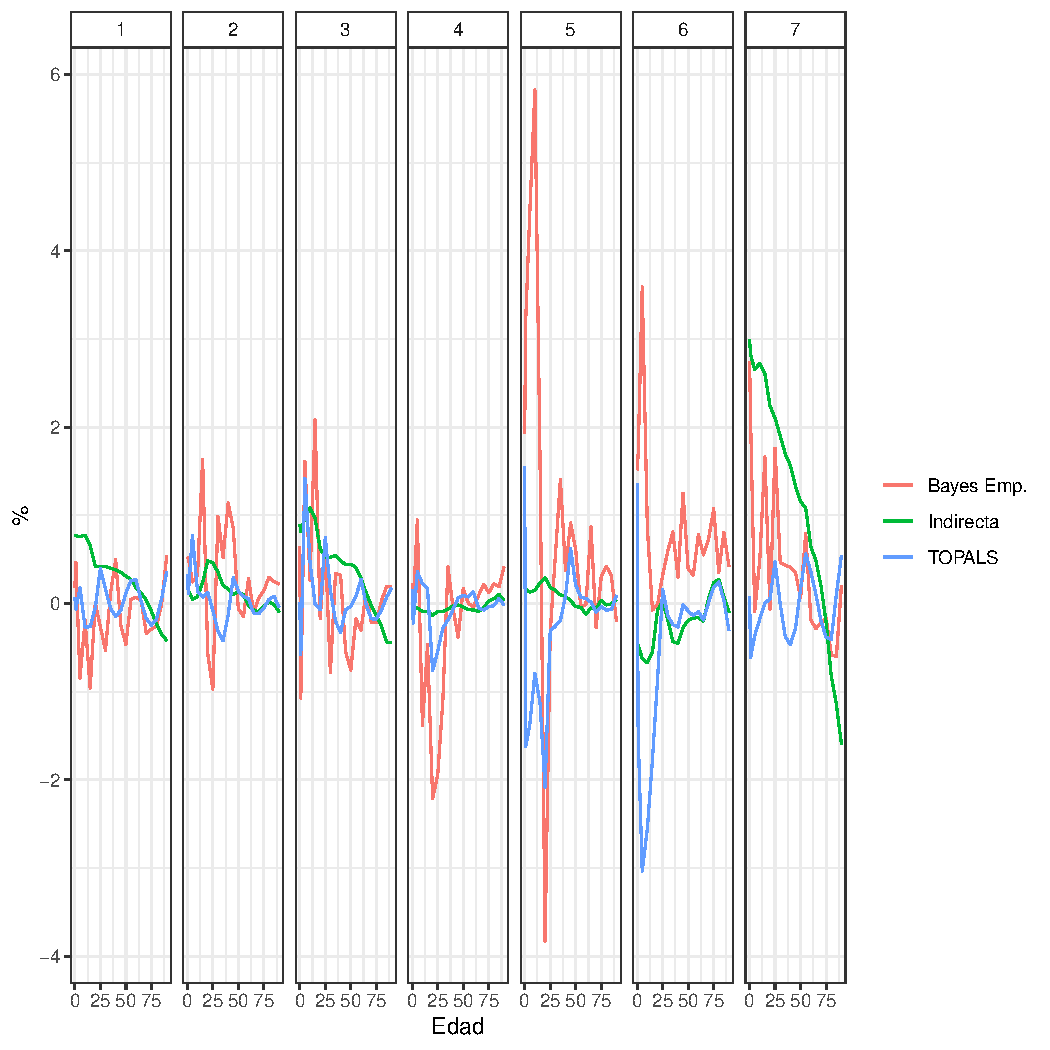
\includegraphics[width=0.7\linewidth]{/Users/nicosacco/GitHub/academicos/research/SubnMort/analysis/plots/ConsistAM} 

}

\caption{Defunciones esperadas respecto a registradas en áreas mayores definidas. Diferencias relativas en porcentaje. Fuente: elaboración porpia}\label{fig:consistAM}
\end{figure}

\begin{landscape}
\begin{longtable}[t]{llrrrr}
\caption{\label{tab:table_e0}Estimación de la esperanza de vida al nacer según método. Departamentos de la Región Pampeana. Años 2009-2010}\\
\toprule
\multicolumn{1}{c}{ } & \multicolumn{1}{c}{ } & \multicolumn{1}{c}{ } & \multicolumn{3}{c}{e(0)} \\
\cmidrule(l{3pt}r{3pt}){4-6}
Provincia & Departmento & Región & BE & Ind & TOPALS\\
\midrule
\endfirsthead
\caption[]{Estimación de la esperanza de vida al nacer según método. Departamentos de la Región Pampeana. Años 2009-2010 \textit{(continued)}}\\
\toprule
Provincia & Departmento & Región & BE & Ind & TOPALS\\
\midrule
\endhead
\
\endfoot
\bottomrule
\endlastfoot
Buenos Aires & 25 de Mayo & 2 & 76.0 & 76.1 & 76.1\\
Buenos Aires & 9 de Julio & 2 & 76.5 & 76.0 & 76.5\\
Buenos Aires & Adolfo Alsina & 6 & 76.4 & 76.5 & 76.3\\
Buenos Aires & Adolfo Gonzales Chaves & 5 & 77.1 & 77.1 & 77.2\\
Buenos Aires & Alberti & 2 & 76.8 & 77.9 & 77.2\\
\addlinespace
Buenos Aires & Almirante Brown & 1 & 74.6 & 74.5 & 74.6\\
Buenos Aires & Arrecifes & 2 & 74.9 & 74.7 & 74.7\\
Buenos Aires & Avellaneda & 1 & 73.3 & 73.7 & 73.2\\
Buenos Aires & Ayacucho & 2 & 76.5 & 77.1 & 76.6\\
Buenos Aires & Azul & 2 & 76.3 & 75.9 & 76.3\\
\addlinespace
Buenos Aires & Bahía Blanca & 5 & 76.8 & 76.8 & 76.7\\
Buenos Aires & Balcarce & 2 & 76.8 & 76.9 & 77.0\\
Buenos Aires & Baradero & 2 & 73.9 & 74.1 & 73.5\\
Buenos Aires & Benito Juárez & 2 & 75.5 & 75.4 & 75.4\\
Buenos Aires & Berazategui & 1 & 74.3 & 74.3 & 74.3\\
\addlinespace
Buenos Aires & Berisso & 1 & 74.1 & 73.8 & 74.0\\
Buenos Aires & Bolívar & 2 & 76.2 & 76.4 & 76.2\\
Buenos Aires & Bragado & 2 & 75.6 & 75.9 & 75.5\\
Buenos Aires & Brandsen & 1 & 75.3 & 75.7 & 75.9\\
Buenos Aires & Campana & 7 & 75.1 & 75.2 & 75.1\\
\addlinespace
Buenos Aires & Cañuelas & 1 & 74.5 & 74.7 & 74.6\\
Buenos Aires & Capitán Sarmiento & 2 & 75.4 & 75.2 & 75.5\\
Buenos Aires & Carlos Casares & 2 & 75.6 & 76.0 & 75.2\\
Buenos Aires & Carlos Tejedor & 2 & 76.8 & 77.6 & 77.7\\
Buenos Aires & Carmen de Areco & 2 & 75.7 & 75.7 & 75.7\\
\addlinespace
Buenos Aires & Castelli & 2 & 75.8 & 76.0 & 75.7\\
Buenos Aires & Chacabuco & 2 & 75.5 & 75.2 & 75.6\\
Buenos Aires & Chascomús & 2 & 79.3 & 80.2 & 80.1\\
Buenos Aires & Chivilcoy & 2 & 76.2 & 76.0 & 76.2\\
Buenos Aires & Colón & 2 & 76.0 & 76.3 & 75.9\\
\addlinespace
Buenos Aires & Coronel de Marina Leonardo Rosales & 5 & 76.7 & 76.6 & 76.8\\
Buenos Aires & Coronel Dorrego & 5 & 77.7 & 78.5 & 78.2\\
Buenos Aires & Coronel Pringles & 5 & 76.0 & 75.8 & 75.8\\
Buenos Aires & Coronel Suárez & 5 & 77.0 & 76.9 & 77.0\\
Buenos Aires & Daireaux & 2 & 76.2 & 76.1 & 76.6\\
\addlinespace
Buenos Aires & Dolores & 2 & 75.4 & 75.3 & 75.2\\
Buenos Aires & Ensenada & 1 & 74.0 & 73.7 & 73.9\\
Buenos Aires & Escobar & 7 & 75.4 & 75.3 & 75.3\\
Buenos Aires & Esteban Echeverría & 1 & 74.5 & 74.6 & 74.6\\
Buenos Aires & Exaltación de la Cruz & 7 & 74.8 & 74.9 & 74.9\\
\addlinespace
Buenos Aires & Ezeiza & 1 & 74.4 & 74.4 & 74.3\\
Buenos Aires & Florencio Varela & 1 & 73.7 & 73.7 & 73.7\\
Buenos Aires & Florentino Ameghino & 2 & 76.1 & 76.4 & 77.0\\
Buenos Aires & General Alvarado & 2 & 76.7 & 76.9 & 77.0\\
Buenos Aires & General Alvear & 2 & 76.1 & 76.2 & 76.6\\
\addlinespace
Buenos Aires & General Arenales & 2 & 75.2 & 75.6 & 74.7\\
Buenos Aires & General Belgrano & 2 & 76.0 & 75.9 & 76.0\\
Buenos Aires & General Guido & 2 & 76.0 & 77.6 & 76.9\\
Buenos Aires & General Juan Madariaga & 2 & 75.7 & 75.7 & 75.5\\
Buenos Aires & General La Madrid & 5 & 76.5 & 76.9 & 76.7\\
\addlinespace
Buenos Aires & General Las Heras & 2 & 75.5 & 75.7 & 75.1\\
Buenos Aires & General Lavalle & 2 & 75.0 & 74.1 & 73.1\\
Buenos Aires & General Paz & 2 & 75.9 & 76.3 & 76.2\\
Buenos Aires & General Pinto & 2 & 75.9 & 75.6 & 76.1\\
Buenos Aires & General Pueyrredón & 2 & 75.7 & 75.7 & 75.7\\
\addlinespace
Buenos Aires & General Rodríguez & 1 & 73.0 & 72.8 & 72.7\\
Buenos Aires & General San Martín & 7 & 74.8 & 74.8 & 74.9\\
Buenos Aires & General Viamonte & 2 & 76.7 & 76.8 & 76.9\\
Buenos Aires & General Villegas & 2 & 76.1 & 76.0 & 76.2\\
Buenos Aires & Guaminí & 5 & 78.4 & 79.6 & 79.4\\
\addlinespace
Buenos Aires & Hipólito Yrigoyen & 2 & 76.5 & 76.5 & 77.1\\
Buenos Aires & Hurlingham & 7 & 76.1 & 76.2 & 76.0\\
Buenos Aires & Ituzaingó & 7 & 76.6 & 76.6 & 76.8\\
Buenos Aires & José C. Paz & 7 & 73.7 & 73.8 & 73.7\\
Buenos Aires & Junín & 2 & 75.2 & 74.9 & 75.1\\
\addlinespace
Buenos Aires & La Costa & 2 & 76.5 & 76.7 & 76.5\\
Buenos Aires & La Plata & 1 & 75.4 & 75.3 & 75.4\\
Buenos Aires & Lanús & 1 & 74.9 & 74.8 & 74.9\\
Buenos Aires & Laprida & 5 & 76.3 & 76.0 & 75.7\\
Buenos Aires & Las Flores & 2 & 76.3 & 76.4 & 76.6\\
\addlinespace
Buenos Aires & Leandro N. Alem & 2 & 75.3 & 76.2 & 74.6\\
Buenos Aires & Lincoln & 2 & 76.0 & 75.7 & 76.1\\
Buenos Aires & Lobería & 2 & 76.9 & 77.1 & 77.4\\
Buenos Aires & Lobos & 2 & 75.9 & 76.3 & 75.7\\
Buenos Aires & Lomas de Zamora & 1 & 74.1 & 74.3 & 74.1\\
\addlinespace
Buenos Aires & Luján & 1 & 74.5 & 74.7 & 74.5\\
Buenos Aires & Magdalena & 2 & 74.9 & 74.5 & 74.6\\
Buenos Aires & Maipú & 2 & 74.8 & 74.4 & 74.0\\
Buenos Aires & Malvinas Argentinas & 7 & 74.4 & 74.5 & 74.5\\
Buenos Aires & Mar Chiquita & 2 & 77.2 & 77.2 & 77.7\\
\addlinespace
Buenos Aires & Marcos Paz & 1 & 73.4 & 73.2 & 73.1\\
Buenos Aires & Mercedes & 7 & 75.1 & 75.2 & 74.9\\
Buenos Aires & Merlo & 1 & 74.2 & 74.1 & 74.2\\
Buenos Aires & Monte & 2 & 74.4 & 74.4 & 73.8\\
Buenos Aires & Monte Hermoso & 5 & 77.2 & 78.2 & 77.8\\
\addlinespace
Buenos Aires & Moreno & 7 & 73.5 & 73.5 & 73.5\\
Buenos Aires & Morón & 7 & 75.2 & 75.1 & 75.3\\
Buenos Aires & Navarro & 2 & 76.1 & 76.3 & 76.1\\
Buenos Aires & Necochea & 2 & 75.9 & 75.8 & 75.9\\
Buenos Aires & Olavarría & 2 & 76.3 & 75.8 & 76.4\\
\addlinespace
Buenos Aires & Patagones & 5 & 77.1 & 77.4 & 77.2\\
Buenos Aires & Pehuajó & 2 & 75.7 & 75.8 & 75.7\\
Buenos Aires & Pellegrini & 5 & 76.1 & 76.2 & 75.8\\
Buenos Aires & Pergamino & 2 & 74.8 & 75.6 & 74.6\\
Buenos Aires & Pila & 2 & 75.0 & 75.1 & 73.7\\
\addlinespace
Buenos Aires & Pilar & 7 & 75.3 & 75.4 & 75.4\\
Buenos Aires & Pinamar & 2 & 76.7 & 77.1 & 77.0\\
Buenos Aires & Presidente Perón & 1 & 72.9 & 72.6 & 72.5\\
Buenos Aires & Puán & 5 & 77.3 & 77.1 & 77.7\\
Buenos Aires & Punta Indio & 2 & 76.7 & 77.1 & 77.4\\
\addlinespace
Buenos Aires & Quilmes & 1 & 74.7 & 74.7 & 74.7\\
Buenos Aires & Ramallo & 2 & 74.8 & 74.7 & 74.6\\
Buenos Aires & Rauch & 2 & 77.1 & 76.9 & 77.9\\
Buenos Aires & Rivadavia & 2 & 75.6 & 75.4 & 75.5\\
Buenos Aires & Rojas & 2 & 75.6 & 75.3 & 75.3\\
\addlinespace
Buenos Aires & Roque Pérez & 2 & 76.4 & 76.8 & 76.7\\
Buenos Aires & Saavedra & 5 & 76.4 & 76.2 & 76.3\\
Buenos Aires & Saladillo & 2 & 77.5 & 77.6 & 78.0\\
Buenos Aires & Salliqueló & 5 & 76.0 & 75.6 & 76.1\\
Buenos Aires & Salto & 2 & 75.3 & 75.3 & 75.2\\
\addlinespace
Buenos Aires & San Andrés de Giles & 7 & 74.5 & 74.6 & 74.1\\
Buenos Aires & San Antonio de Areco & 2 & 75.9 & 75.7 & 76.1\\
Buenos Aires & San Cayetano & 5 & 77.1 & 77.0 & 77.3\\
Buenos Aires & San Fernando & 7 & 74.4 & 74.5 & 74.3\\
Buenos Aires & San Isidro & 7 & 77.2 & 76.9 & 77.2\\
\addlinespace
Buenos Aires & San Miguel & 7 & 75.0 & 75.0 & 75.0\\
Buenos Aires & San Nicolás & 2 & 75.4 & 75.4 & 75.3\\
Buenos Aires & San Pedro & 2 & 73.9 & 74.0 & 73.6\\
Buenos Aires & San Vicente & 1 & 74.0 & 73.8 & 73.9\\
Buenos Aires & Suipacha & 2 & 76.1 & 76.1 & 76.2\\
\addlinespace
Buenos Aires & Tandil & 2 & 77.1 & 76.7 & 77.2\\
Buenos Aires & Tapalqué & 2 & 76.4 & 76.8 & 77.1\\
Buenos Aires & Tigre & 7 & 75.0 & 75.0 & 75.1\\
Buenos Aires & Tordillo & 2 & 75.6 & 74.2 & 74.7\\
Buenos Aires & Tornquist & 5 & 78.6 & 78.9 & 80.0\\
\addlinespace
Buenos Aires & Trenque Lauquen & 2 & 76.6 & 75.8 & 76.8\\
Buenos Aires & Tres Arroyos & 5 & 76.4 & 76.3 & 76.4\\
Buenos Aires & Tres de Febrero & 7 & 75.0 & 74.9 & 75.1\\
Buenos Aires & Tres Lomas & 5 & 77.7 & 78.6 & 78.7\\
Buenos Aires & Vicente López & 7 & 78.3 & 77.8 & 78.6\\
\addlinespace
Buenos Aires & Villa Gesell & 2 & 75.5 & 75.0 & 75.4\\
Buenos Aires & Villarino & 5 & 75.8 & 75.9 & 75.5\\
Buenos Aires & Zárate & 7 & 74.6 & 74.6 & 74.5\\
Córdoba & Calamuchita & 4 & 77.6 & 78.1 & 78.0\\
Córdoba & Capital & 4 & 76.1 & 76.1 & 76.1\\
\addlinespace
Córdoba & Colón & 4 & 75.9 & 75.7 & 76.0\\
Córdoba & Cruz del Eje & 4 & 75.8 & 76.1 & 75.6\\
Córdoba & General Roca & 6 & 77.0 & 77.2 & 77.2\\
Córdoba & General San Martín & 6 & 74.8 & 74.7 & 74.9\\
Córdoba & Ischilín & 4 & 76.1 & 76.4 & 76.0\\
\addlinespace
Córdoba & Juárez Celman & 6 & 76.6 & 76.4 & 76.6\\
Córdoba & Marcos Juárez & 2 & 77.2 & 76.7 & 77.4\\
Córdoba & Minas & 4 & 75.9 & 76.4 & 75.5\\
Córdoba & Pocho & 4 & 77.3 & 82.1 & 81.5\\
Córdoba & Presidente Roque Sáenz Peña & 2 & 76.6 & 76.5 & 76.9\\
\addlinespace
Córdoba & Punilla & 4 & 76.2 & 76.0 & 76.2\\
Córdoba & Río Cuarto & 6 & 75.9 & 75.7 & 75.9\\
Córdoba & Río Primero & 4 & 76.4 & 76.7 & 76.7\\
Córdoba & Río Seco & 4 & 75.2 & 75.1 & 73.9\\
Córdoba & Río Segundo & 4 & 75.9 & 75.5 & 75.9\\
\addlinespace
Córdoba & San Alberto & 4 & 77.2 & 78.1 & 77.7\\
Córdoba & San Javier & 4 & 75.1 & 74.9 & 74.6\\
Córdoba & San Justo & 4 & 75.5 & 75.3 & 75.5\\
Córdoba & Santa María & 4 & 76.5 & 76.2 & 76.7\\
Córdoba & Sobremonte & 4 & 74.1 & 70.2 & 70.8\\
\addlinespace
Córdoba & Tercero Arriba & 4 & 75.7 & 75.9 & 75.6\\
Córdoba & Totoral & 4 & 76.4 & 76.8 & 76.7\\
Córdoba & Tulumba & 4 & 76.4 & 77.4 & 76.8\\
Córdoba & Unión & 4 & 75.9 & 75.9 & 76.0\\
Entre Ríos & Colón & 3 & 75.4 & 75.1 & 75.4\\
\addlinespace
Entre Ríos & Concordia & 3 & 73.9 & 73.8 & 73.8\\
Entre Ríos & Diamante & 3 & 75.7 & 75.9 & 75.8\\
Entre Ríos & Federación & 3 & 75.1 & 75.2 & 75.1\\
Entre Ríos & Federal & 3 & 74.2 & 74.5 & 74.1\\
Entre Ríos & Feliciano & 3 & 73.7 & 73.5 & 72.9\\
\addlinespace
Entre Ríos & Gualeguay & 3 & 74.9 & 75.2 & 74.8\\
Entre Ríos & Gualeguaychú & 3 & 75.7 & 75.5 & 75.7\\
Entre Ríos & Islas del Ibicuy & 7 & 75.6 & 75.9 & 75.6\\
Entre Ríos & La Paz & 3 & 74.0 & 73.5 & 73.8\\
Entre Ríos & Nogoyá & 3 & 75.5 & 75.6 & 75.4\\
\addlinespace
Entre Ríos & Paraná & 3 & 75.7 & 75.5 & 75.7\\
Entre Ríos & San Salvador & 3 & 75.7 & 75.8 & 75.7\\
Entre Ríos & Tala & 3 & 75.2 & 75.6 & 75.3\\
Entre Ríos & Uruguay & 3 & 75.9 & 75.7 & 76.0\\
Entre Ríos & Victoria & 3 & 75.8 & 75.9 & 75.7\\
\addlinespace
Entre Ríos & Villaguay & 3 & 75.4 & 75.8 & 75.4\\
La Pampa & Atreucó & 6 & 75.5 & 75.9 & 75.4\\
La Pampa & Caleu Caleu & 5 & 77.5 & 83.3 & 83.4\\
La Pampa & Capital & 6 & 76.6 & 76.8 & 76.7\\
La Pampa & Catriló & 6 & 77.7 & 78.6 & 78.1\\
\addlinespace
La Pampa & Chalileo & 6 & 78.2 & 84.1 & 84.2\\
La Pampa & Chapaleufú & 6 & 76.8 & 77.0 & 77.1\\
La Pampa & Chical Co & 6 & 76.9 & 81.8 & 81.3\\
La Pampa & Conhelo & 6 & 76.4 & 77.0 & 76.5\\
La Pampa & Curacó & 6 & 76.7 & 80.7 & 80.9\\
\addlinespace
La Pampa & Guatraché & 6 & 77.1 & 77.5 & 77.7\\
La Pampa & Hucal & 5 & 77.0 & 76.8 & 76.9\\
La Pampa & Lihuel Calel & 5 & 77.1 & 82.7 & 82.6\\
La Pampa & Limay Mahuida & 6 & 75.9 & 76.0 & 75.1\\
La Pampa & Limay Mahuida & 6 & 75.9 & 76.0 & 75.1\\
\addlinespace
La Pampa & Loventué & 6 & 76.3 & 76.8 & 76.9\\
La Pampa & Maracó & 6 & 76.4 & 77.0 & 76.3\\
La Pampa & Puelén & 6 & 78.0 & 79.6 & 80.0\\
La Pampa & Quemú Quemú & 6 & 77.0 & 77.9 & 77.5\\
La Pampa & Rancul & 6 & 76.7 & 76.7 & 77.4\\
\addlinespace
La Pampa & Realicó & 6 & 77.3 & 77.2 & 77.8\\
La Pampa & Toay & 6 & 77.1 & 77.7 & 78.2\\
La Pampa & Trenel & 6 & 77.1 & 78.6 & 78.7\\
La Pampa & Utracán & 6 & 76.0 & 76.8 & 75.9\\
Santa Fe & 9 de Julio & 3 & 74.4 & 74.7 & 74.4\\
\addlinespace
Santa Fe & Belgrano & 2 & 76.0 & 76.1 & 76.1\\
Santa Fe & Caseros & 3 & 76.7 & 76.4 & 76.9\\
Santa Fe & Castellanos & 3 & 76.7 & 76.3 & 76.8\\
Santa Fe & Constitución & 2 & 76.7 & 76.7 & 76.8\\
Santa Fe & Garay & 3 & 74.6 & 74.7 & 74.4\\
\addlinespace
Santa Fe & General López & 2 & 75.8 & 75.9 & 75.8\\
Santa Fe & General Obligado & 3 & 75.0 & 75.2 & 75.0\\
Santa Fe & Iriondo & 2 & 75.4 & 75.4 & 75.4\\
Santa Fe & La Capital & 3 & 74.7 & 74.8 & 74.7\\
Santa Fe & Las Colonias & 3 & 76.7 & 76.4 & 76.9\\
\addlinespace
Santa Fe & Rosario & 2 & 75.1 & 75.3 & 75.1\\
Santa Fe & San Cristóbal & 3 & 75.1 & 75.3 & 74.9\\
Santa Fe & San Javier & 3 & 73.6 & 73.9 & 73.3\\
Santa Fe & San Jerónimo & 3 & 75.5 & 75.3 & 75.4\\
Santa Fe & San Justo & 3 & 75.4 & 75.4 & 75.4\\
\addlinespace
Santa Fe & San Lorenzo & 3 & 75.6 & 75.5 & 75.7\\
Santa Fe & San Martín & 2 & 76.8 & 77.2 & 76.9\\
Santa Fe & Vera & 3 & 73.3 & 73.8 & 73.3\\*
\end{longtable}
\end{landscape}

\hypertarget{referencias}{%
\section*{Referencias}\label{referencias}}
\addcontentsline{toc}{section}{Referencias}

\hypertarget{refs}{}
\leavevmode\hypertarget{ref-Alexander2017}{}%
Alexander, Monica, Emilio Zagheni, y Magali Barbieri. 2017. «A Flexible
Bayesian Model for Estimating Subnational Mortality». \emph{Demography}
54 (6). NIH Public Access: 2025.
\url{https://doi.org/10.1007/s13524-017-0618-7}.

\leavevmode\hypertarget{ref-Arriaga2011}{}%
Arriaga, E. 2011. \emph{Análisis demográfico de la mortalidad}.
Universidad Nacional de Córdoba.

\leavevmode\hypertarget{ref-AssunCao2006}{}%
Assuncao, R. M., M. C. Neves, G. Camara, y C. Da Costa Freitas. 2006.
«Efficient regionalization techniques for socio-economic geographical
units using minimum spanning trees». \emph{International Journal of
Geographical Information Science} 20 (7). Taylor \& Francis: 797-811.
\url{https://doi.org/10.1080/13658810600665111}.

\leavevmode\hypertarget{ref-Assuncao2005}{}%
Assunção, Renato M., Carl P. Schmertmann, Joseph E. Potter, y Suzana M.
Cavenaghi. 2005. «Empirical Bayes Estimation of Demographic Schedules
for Small Areas». \emph{Demography} 42 (3). Springer: 537-58.
\url{http://www.jstor.org/stable/4147361}.

\leavevmode\hypertarget{ref-deBeer2011}{}%
Beer, Joop de. 2011. «A new relational method for smoothing and
projecting age-specific fertility rates: TOPALS». \emph{Demographic
Research} 24 (marzo). Demographic Research: 409-54.
\url{https://www.demographic-research.org/volumes/vol24/18/default.htm}.

\leavevmode\hypertarget{ref-Bennett_Horiuchi_1984}{}%
Bennett, Neil G, y Shiro Horiuchi. 1984. «Mortality Estimation from
Registered Deaths in Less Developed Countries». \emph{Demography} 21
(2). Springer: 217-33. \url{https://doi.org/10.2307/2061041}.

\leavevmode\hypertarget{ref-Bivand2019}{}%
Bivand, Roger. 2019. «Spatial Dependence: Weighting Schemes, Statistics
and Models {[}R package spdep version 1.1-2{]}». Comprehensive R Archive
Network (CRAN).
\url{https://cran.r-project.org/web/packages/spdep/index.html}.

\leavevmode\hypertarget{ref-Borges2018}{}%
Borges, Gabriel. 2018. «Teorías y medidas de convergencia demográfica:
una aplicación a nivel subnacional en América Latina». \emph{Notas de
Población}, n.º 106: 37-64.

\leavevmode\hypertarget{ref-Borges2017}{}%
Borges, Gabriel Mendes. 2017. «Health transition in Brazil: regional
variations and divergence/convergence in mortality». \emph{Cadernos de
SaÃPÃ} 33 (0). scielo.
\url{http://www.scielo.br/scielo.php?script=sci_arttext\&pid=S0102-311X2017000805001\&nrm=iso}.

\leavevmode\hypertarget{ref-Brillinger1986}{}%
Brillinger, D. R. 1986. «The natural variability of vital rates and
associated statistics». \emph{PubMed. comprises. more. than. 29 million.
citations. for. biomedical. literature. from. MEDLINE, life. science.
journals., and. online. books.} 42 (4). Wiley: 693-734.
\url{https://www.ncbi.nlm.nih.gov/pubmed/3814721}.

\leavevmode\hypertarget{ref-Camisa1964}{}%
Camisa, Zulma C. 1964. «Tabla abreviada de mortalidad de la region
pampeana de la Republica Argentina 1946-1948; precedida de un analisis
critico de las estadisticas basicas». \emph{Repec.org}.
\url{https://econpapers.repec.org/paper/ecrcol048/8246.htm}.

\leavevmode\hypertarget{ref-DEIS2016}{}%
DEIS. 2016. Ministerio de Slaud de la Nación.
\url{http://www.deis.msal.gov.ar/wp-content/uploads/2016/09/Estadisticasvitales2016.pdf}.

\leavevmode\hypertarget{ref-Efron1972}{}%
Efron, Bradley, y Carl Morris. 1972. «Empirical Bayes on Vector
Observations: An Extension of Stein's Method». \emph{Biometrika} 59 (2).
{[}Oxford University Press, Biometrika Trust{]}: 335-47.
\url{http://www.jstor.org/stable/2334578}.

\leavevmode\hypertarget{ref-Fenelon2013}{}%
Fenelon, Andrew. 2013. «Geographic divergence in mortality in the United
States». \emph{Population and development review} 39 (4): 611-34.

\leavevmode\hypertarget{ref-FreireEtAl2015}{}%
Freire, Queiroz, F. H. M. d. A. 2015. «Mortality Estimates and
Construction of Life Tables for Small Areas in Brazil, 2010».

\leavevmode\hypertarget{ref-GeriMoscoso2018}{}%
GERI, Fernando; MOSCOSO, Milva; LAGO. 2018. «Bonos demográficos en
Argentina, 1960-2015». \emph{Estudios demográficos y urbanos} 33 (1):
225-52.

\leavevmode\hypertarget{ref-GonzagaSchmertmann2016}{}%
Gonzaga, Carl Paul, Marcos R.; Schmertmann. 2016. «Estimativa de taxas
de mortalidade por idade e sexo para pequenas áreas com regressão de
TOPALS: uma aplicação para o Brasil em 2010». \emph{Revista Brasileira
De Estudos De População} 33 (12): 629-52.

\leavevmode\hypertarget{ref-Gonzaga_Schmertmann_2016}{}%
Gonzaga, Marcos R., y Carl Paul Schmertmann. 2016. «Estimating age- and
sex-specific mortality rates for small areas with TOPALS regression: an
application to Brazil in 2010». \emph{Revista Brasileira de Estudos de
População} 33 (3): 629-52.
\url{https://doi.org/10.20947/s0102-30982016c0009}.

\leavevmode\hypertarget{ref-Gragnolati2015}{}%
Gragnolati, Rafael P.; Apella, Michele; Rofman. 2015. \emph{As time goes
by in Argentina : economic opportunities and challenges of the
demographic transition}. World Bank Publications.

\leavevmode\hypertarget{ref-Grushka2013}{}%
Grushka, Baum, C. 2013. «Vivir y morir en las comunas de la Ciudad de
Buenos Aires: un estudio de diferenciales». Población de Buenos Aires.

\leavevmode\hypertarget{ref-INDEC2013}{}%
INDEC. 2013. «Tablas abreviadas de mortalidad por sexo y edad 2008-2010:
total del país y provincias».

\leavevmode\hypertarget{ref-INDEC2015}{}%
---------. 2015. «Estimaciones de población por sexo, departamento y año
calendario2010-2025».

\leavevmode\hypertarget{ref-James2014}{}%
James, Gareth, Daniela Witten, Trevor Hastie, y Robert Tibshirani. 2014.
\emph{An Introduction to Statistical Learning: With Applications in R}.
Springer Publishing Company, Incorporated.

\leavevmode\hypertarget{ref-JaspersOrellana1994}{}%
Jaspers, D., y H. Orellana. 1994. «Evaluación del uso de las
estadísticas vitales para estudios de causas de muerte en América
Latina». \emph{Notas de Población} 60 (CELADE): 47-77.

\leavevmode\hypertarget{ref-Kaztman1995}{}%
Kaztman, Rubén. 1995. «La medición de las necesidades básicas
insatisfechas en los censos de población». Centro Latinoamericano de
Demografía.

\leavevmode\hypertarget{ref-LimaQueiroz2014}{}%
Lima, Everton Emanuel Campos de, y Bernardo Lanza Queiroz. 2014.
«Evolution of the deaths registry system in Brazil: associations with
changes in the mortality profile, under-registration of death counts,
and ill-defined causes of death». \emph{Cadernos de Saúde Pública} 30
(8): 1721-30.
\url{https://doi.org/https://dx.doi.org/10.1590/0102-311X00131113}.

\leavevmode\hypertarget{ref-Longford2005}{}%
Longford, Nicholas T. 2005. \emph{Missing Data and Small-Area Estimation
- Modern Analytical Equipment for the Survey Statistician}.
\emph{Springer.com}.
\url{https://www.springer.com/gp/book/9781852337605}.

\leavevmode\hypertarget{ref-Longford1999}{}%
Longford, N. T. 1999. «Multivariate shrinkage estimation of small area
means and proportions». \emph{Journal of the Royal Statistical Society:
Series A (Statistics in Society)} 162 (2): 227-45.
\url{https://doi.org/10.1111/1467-985X.00132}.

\leavevmode\hypertarget{ref-Luy2010}{}%
Luy, Marc. 2010. «A classification of the nature of mortality data
underlying the estimates for the 2004 and 2006 United Nations World
Population Prospects». \emph{Comparative Population Studies} 35 (2):
73-100.

\leavevmode\hypertarget{ref-Marshall1991}{}%
Marshall, Roger J. 1991. «Mapping Disease and Mortality Rates Using
Empirical Bayes Estimators». \emph{Journal of the Royal Statistical
Society. Series C (Applied Statistics)} 40 (2). {[}Wiley, Royal
Statistical Society{]}: 283-94.
\url{http://www.jstor.org/stable/2347593}.

\leavevmode\hypertarget{ref-Matthews2013}{}%
Matthews S.A.; Parker, D.M. 2013. «Progress in spatial demography».
\emph{Demographic Research}, n.º 28: 271-312.

\leavevmode\hypertarget{ref-Miech2011}{}%
Miech, Pampel; Jinyoung, Richard; Fred. 2011. «The Enduring Association
between Education and Mortality:The Role of Wideningand Narrowing
Disparities». \emph{American Sociological Review}, n.º 76: 913-34.

\leavevmode\hypertarget{ref-Moultrie}{}%
Moultrie, Tom, RE Dorrington, A G Hill, K H Hill, Ian Timaeus, y Basia
Zaba. 2013. \emph{Tools for Demographic Estimation}.

\leavevmode\hypertarget{ref-Otero2012}{}%
Otero, Hernán, ed. 2012. \emph{Historia de la provincia de Buenos Aires.
Población, ambiente y territorio, Buenos Aires,} UNIPE-Edhasa,

\leavevmode\hypertarget{ref-Peralta2019}{}%
Peralta, Joan; Borrell, Andrés; Benach. 2019. «Evolution of the deaths
registry system in Brazil: associations with changes in the mortality
profile, under-registration of death counts, and ill-defined causes of
death». \emph{Population Health Metric} 17 (3): 3.

\leavevmode\hypertarget{ref-Preston1975}{}%
Preston, Samuel H. 1975. «The Changing Relation between Mortality and
Level of Economic Development». \emph{Population Studies} 29 (2).
{[}Population Investigation Committee, Taylor; Francis, Ltd.{]}: 231-48.
\url{https://doi.org/10.2307/2173509}.

\leavevmode\hypertarget{ref-Preston1980}{}%
Preston, Samuel, Ansley J. Coale, James Trussell, y Maxine Weinstein.
1980. «Estimating the Completeness of Reporting of Adult Deaths in
Populations That Are Approximately Stable». \emph{Population index} 46
(febrero): 179-202. \url{https://doi.org/10.2307/2736122}.

\leavevmode\hypertarget{ref-Robbins1983}{}%
Robbins, Herbert. 1983. «Some Thoughts on Empirical Bayes Estimation».
\emph{The Annals of Statistics} 11 (3). Institute of Mathematical
Statistics: 713-23. \url{http://www.jstor.org/stable/2240635}.

\leavevmode\hypertarget{ref-SaccoBorges2018}{}%
Sacco, G., N.; Borges. 2018. «¿Converge la fecundidad en Brasil y
Argentina? Un enfoque desde las desigualdades». \emph{Revista Brasileira
de Estudos de População} 35 (1).

\leavevmode\hypertarget{ref-Sacco2016}{}%
Sacco, Nicolás. 2016. «¿Cuánto vivieron los nacidos a fines del siglo
XIX y cuánto vivirán los nacidos a fines del siglo XX?» \emph{Notas de
Población} 103 (julio-diciembre): 73-100.

\leavevmode\hypertarget{ref-Schmertmann2018}{}%
Schmertmann, Carl Paul, y Marcos R. Gonzaga. 2018. «Bayesian Estimation
of Age-Specific Mortality and Life Expectancy for Small Areas With
Defective Vital Records». \emph{Demography} 55 (4): 1363-88.
\url{https://doi.org/10.1007/s13524-018-0695-2}.

\leavevmode\hypertarget{ref-Torcida2008}{}%
Torcida, Sebastián, Andrea L Vega, y Guillermo A Velázquez. 2008.
«Análisis de la Evolución de la Tasa de Mortalidad Infantil en los
Departamentos de Argentina. 1994-20».

\leavevmode\hypertarget{ref-Bilal2019}{}%
Usama Bilal, Waleska T. Caiaffa, Marcio Alazraqui. 2019. «Inequalities
in life expectancy in six large Latin American cities from the SALURBAL
study: an ecological analysis». \emph{The Lancet Planetary Health} 3
(12): e503-e510.

\leavevmode\hypertarget{ref-Wrycza2012}{}%
Wrycza, Tomasz, y Annette Baudisch. 2012. «How life expectancy varies
with perturbations in age-specific mortality». \emph{Demographic
Research} 27 (septiembre). Demographic Research: 365-76.
\url{https://www.demographic-research.org/volumes/vol27/13/default.htm}.

\end{document}
